%==================================================================================================
% LaTeX paper template - use as a starting point for structuring a research paper.
%
% Written by Colin Perkins (https://csperkins.org/)
% 2002-2018
%
% To the extent possible under law, the author(s) have dedicated all copyright and
% related and neighbouring rights to this software to the public domain worldwide.
% This template is distributed without any warranty.
%
% You should have received a copy of the CC0 Public Domain Dedication along with
% this software. If not, see <http://creativecommons.org/publicdomain/zero/1.0/>.
%
% NOTE: The above Public Domain Dedication applies only to the LaTeX paper
% template distributed from https://github.com/csperkins/project-template
% in the file papers/example.tex. Unless explicitly stated, modifications 
% or additions to that template are copyright by their respective authors.
%==================================================================================================

%==================================================================================================
% General advice on technical writing:
%  - George Gopen and Judith Swan, "The Science of Scientific Writing",
%    American Scientist, Nov/Dec 1990. 
%    http://www.americanscientist.org/issues/num2/the-science-of-scientific-writing/1
%  - Stephen Pinker, "The Sense of Style: The Thinking Person's Guide to
%    Writing in the 21st Century", Penguin, Sept 2014. ISBN 0525427929.
%
% The paper writing advice in the comments is derived from talks and articles
% by Simon Peyton-Jones, Jim Kurose, Henning Schulzrinne, and Jim Bednar: 
%  - http://research.microsoft.com/~simonpj/papers/giving-a-talk/giving-a-talk.htm
%  - http://research.microsoft.com/~simonpj/papers/giving-a-talk/writing-a-paper-slides.pdf
%  - http://gaia.cs.umass.edu/kurose/talks/top_10_tips_for_writing_a_paper.ppt
%  - http://www-net.cs.umass.edu/kurose/writing/intro-style.html
%  - http://www.cs.columbia.edu/~hgs/etc/writing-style.html
%  - http://homepages.inf.ed.ac.uk/jbednar/writingtips.html
%  - http://www.gabbay.org.uk/blog/paper-writing.html
%  - http://homes.cs.washington.edu/~mernst/advice/write-technical-paper.html
%  - http://dx.doi.org/10.1371/journal.pcbi.1005619
%
% LaTeX usage notes:
%  - http://www.read.seas.harvard.edu/~kohler/latex.html
%
%==================================================================================================

%==================================================================================================
% The \documentclass{} macro specifies the overall style. For computer
% networking papers, common options are:
%
%   \documentclass[twocolumn,a4paper]{article}  % Base LaTeX style
%   \documentclass[conference]{IEEEtran}        % IEEE Conference
%   \documentclass[10pt,sigconf]{acmart}        % ACM SIGCOMM conference
%
% The IEEE and ACM templates are included in the lib/tex/inputs directory,
% but check for updates and use the version specified by the conference or
% journal to which you're submitting.

\documentclass[10pt,sigconf]{acmart}
\synctex=1
\graphicspath{{figures/}{doc/paper/}}

% The following packages are recommended, and should be available in most
% standard LaTeX installations (or from https://www.ctan.org/). Note that 
% the order in which packages are loaded is significant.

% Basic extensions recommended for all LaTeX documents:
%   nag        Warn about common problems with LaTeX files
%   inputenc   Specify the character set used in .tex files
%   babel      Language-specific typography and hyphenation
%   microtype  Improved typography when generating PDF files

\usepackage[l2tabu,orthodox]{nag}
\usepackage[utf8x]{inputenc}
\usepackage[british]{babel}
\usepackage{ifpdf}
\usepackage{longtable}
\ifpdf
  \usepackage{microtype}
\fi

% The AMS mathematics library greatly extends and improves mathematics
% support in LaTeX (see http://ctan.org/pkg/amsmath for details). When
%  preparing multi-line numbered equations, be sure to use:
%
%   \begin{align}
%     ...
%   \end{align} 
%
% rather than:
%
%   \begin{eqnarray}
%     ...
%   \end{eqnarray}.  
%
% when this package is loaded, to ensure they formatting is consistent
% (see https://tug.org/pracjourn/2006-4/madsen/madsen.pdf for details).

\usepackage{amsmath}
\usepackage[all]{onlyamsmath}

% Use Times, Helvetica, and Courier fonts, rather than Computer Modern:

\makeatletter
\@ifclassloaded{acmart}{
  % The ACM article style sets the fonts internally
}{
  \usepackage{newtxtext}
  \usepackage{newtxmath}
}
\makeatother

% Add support for sub-figures within a figure, as follows:
%
%   \begin{figure}
%     \centering
%     \subfloat[caption for 1st subfloat]{
%       \includegraphics{...}
%       \label{...}
%     }
%     \\
%     \subfloat[caption for 2nd subfloat]{
%       \includegraphics{...}
%       \label{...}
%     }
%     \caption{caption for entire figure}
%     \label{...}
%   \end{figure*}
%
% The subfig package obsoletes the older subfigure package, and is itself
% deprecated in favour of the subcaption package. However, as of April 2015
% subcaption doesn't work with ACM or IEEE style files (this is also the
% reason for the [caption=false] option).

\usepackage[caption=false]{subfig}

% Improve formatting of tables. To produce nice looking tables:
%
%   - avoid vertical lines;
%   - avoid double horizontal lines;
%   - use horizontal lines above and below the table, and to separate the
%     header from the body of the table, but not elsewhere; and
%   - if in doubt, align columns to the left (columns of numbers should
%     align to the decimal point)
%
% This translates to a tabular environment that looks something like the
% following:
%
%   \begin{tabular}{lll}
%     \toprule
%        Header1 & Header2 & Header3 \\
%     \midrule
%        Line1   & ...     & ...     \\
%        Line2   & ...     & ...     \\
%        Line3   & ...     & ...     \\
%        Line4   & ...     & ...     \\
%     \bottomrule
%   \end{tabular}

\usepackage{booktabs}

% Improve formatting for quote marks in verbatim mode:
\usepackage{upquote}

% Improve support for graphics:
\usepackage{graphicx}

% Add support for URLs using \url{...}. This formats the URL in typewriter
% font, and makes it a hyperlink if the hyperref package is also loaded.
\usepackage{url}

% Add support for drawing packet headers. For instructions, see
% http://ctan.org/tex-archive/macros/latex/contrib/bytefield
\usepackage{bytefield}

% Add support for typesetting program source code. You can either include
% code in-line:
%
%   \begin{lstlisting}[language=Python]
%   Source code goes here
%   \end{lstlisting}
%
% or include a source file:
%
%  \lstinputlisting[language=Python]{source_filename.py}
%
% This package is highly customisable and supports a range of languages.
% See package documentation at https://ctan.org/pkg/listings for details.
\usepackage{listings}

% Generated PDF files can include hyperlinks for URLs and cross-references
% using the hyperref package. This package, however, can interact poorly
% with others. Known issues include:
%
%  - Papers typeset without page numbers gives warnings of the form:
%      "pdfTeX warning (ext4): destination with the same identifier 
%      (name{page.}) has been already used, duplicate ignored".
%    since hyperref tries to refer to the page number.
%  - The algorithmic package uses the same line-numbering scheme for each
%    algorithm, and can cause duplicate identifier warnings if you have
%    several algorithms with line numbers (this may have been fixed with 
%    recent versions of algorithmic...).
%  - If using the algorithm package with hyperref, you need to load packages
%    in the following order (see README in hyperref documentation):
%      \usepackage{float}
%      \usepackage{hyperref}
%      \usepackage{algorithm}
% For these reasons, hyperref is best to avoid for most papers, however if
% needed, uncomment the following two lines:
%  \usepackage{float}
%  \usepackage{hyperref}

% The algorithm package defines the algorithm environment. This is used in
% the same way as the figure and table environments, to include algorithms
% in a paper. The algpseudocode package provides the ability to typeset the
% algorithms: http://ctan.org/tex-archive/macros/latex/contrib/algorithmicx
\usepackage{algorithm}
\usepackage{algpseudocode}
\usepackage{color}


% By default, LaTeX adds extra space after punctuation. The \frenchspacing
% command disables this. This creates tighter looking, more even, text and
% avoids inconsistencies if you forget to use '\ ' to suppress the spacing
% after in-sentence punctuation.
\frenchspacing

% Prevent hyphenation of all upper case words:
\uchyph=0

% The ACM style needs \maketitle after the abstract, but the other styles
% want it before; these macros hide the difference and are used below:
\makeatletter
\@ifclassloaded{acmart}{
  \newcommand{\maketitleSTD}{}
  \newcommand{\maketitleACM}{\maketitle}
}{
  \newcommand{\maketitleSTD}{\maketitle}
  \newcommand{\maketitleACM}{}
}
\makeatother

% Define a simple \todo{...} macro:
\newcommand{\todo}[1]{\textbf{\textcolor{red}{To do: #1}}}

\newcommand{\idea}[1]{{\textcolor{blue}{#1}}}

%==================================================================================================
\begin{document}
% Specify the title of the document:

\title{Does TCP's New Congestion Window Validation Improve HTTP Adaptive Streaming Performance?}

% Specify the authors of the document. Unfortunately, there's no consistent
% way to do this that works across the different document classes. 
%
% If using \documentclass{article}:
%
%   \author{
%      A. N. Other\\University of Glasgow
%   \and
%      Colin Perkins\\University of Glasgow
%   }
%
% If using \documentclass{IEEEtran}:
%
%   \author{
%     \IEEEauthorblockN{A. N. Other}
%     \IEEEauthorblockA{University of Glasgow}
%   \and
%     \IEEEauthorblockN{Colin Perkins}
%     \IEEEauthorblockA{University of Glasgow}
%   }
%
% If using \documentclass{acmart} add a block like the following per author:
%
%   \author{Colin Perkins}
%   \orcid{0000-0002-3404-8964}
%   \affiliation{
%     \institution{University of Glasgow}
%     \streetaddress{School of Computing Science}
%     \city{Glasgow}
%     \postcode{G12 8QQ}
%     \country{UK}
%   }
%   \email{csp@csperkins.org}
%
% If you don't have an ORCID identifier, sign up for one at https://orcid.org

\author{Mihail Yanev}
    %\orcid{0000-0002-3404-8964}
    \affiliation{
      \institution{University of Glasgow}
      \streetaddress{School of Computing Science}
      \city{Glasgow}
      \postcode{G12 8QQ}
      \country{UK}
    }
    \email{m.yanev.1@research.gla.ac.uk}


\author{Stephen McQuistin}
    % \orcid{0000-0002-3404-8964}
    \affiliation{
    \institution{University of Glasgow}
    \streetaddress{School of Computing Science}
    \city{Glasgow}
    \postcode{G12 8QQ}
    \country{UK}
    }
    \email{}

\author{Colin Perkins}
  \orcid{0000-0002-3404-8964}
  \affiliation{
    \institution{University of Glasgow}
    \streetaddress{School of Computing Science}
    \city{Glasgow}
    \postcode{G12 8QQ}
    \country{UK}
  }
  \email{csp@csperkins.org}



% Specify metadata about the paper. Again, what is required depends on the
% document class. If using \documentclass{acmart}, specify the following:
%
%   \acmYear{2018}
%   \copyrightyear{2018}
%   \setcopyright{acmcopyright}
%   \acmConference{CoNEXT '18}{December 4--7, 2018}{Heraklion/Crete, Greece}
%   \acmPrice{15.00}
%   \acmDOI{10.1145/3284850.3284856}
%   \acmISBN{978-1-4503-6082-1/18/12}
%
% The complete metadata is likely only available when preparing the final,
% camera ready, version of the paper.

\acmYear{2021}
\copyrightyear{2021}
\setcopyright{acmcopyright}
\acmConference{MMSys '21}
% {December 4--7, 2018}{Heraklion/Crete, Greece}
\acmPrice{15.00}
% \acmDOI{10.1145/3284850.3284856}
% \acmISBN{978-1-4503-6082-1/18/12}

%==================================================================================================
\maketitleSTD
\begin{abstract}
  % Four sentences:
  %  - State the problem
  %  - Say why it's an interesting problem
  %  - Say what your solution achieves
  %  - Say what follows from your solution

In HTTP video streaming playback stability is an important metric contributing to the user's quality of experience. Throughput adaptive algorithms are known to achieve lower levels of playback stability than their buffer-based counterparts. New congestion window validation is a proposal aiming to keep the transport's transfer rate more stable. This paper shows how this reflects the playback stability. We find that while new congestion window validation stabilises the transfer rate in the transport layer this does not translate to a significant difference in the application's playback stability. 

\end{abstract}
\maketitleACM


\section{Introduction}
\label{sec:introduction}

% A good paper introduction is fairly formulaic. If you follow a simple set
% of rules, you can write a very good introduction. The following outline can
% be varied. For example, you can use two paragraphs instead of one, or you
% can place more emphasis on one aspect of the intro than another. But in all
% cases, all of the points below need to be covered in an introduction, and
% in most papers, you don't need to cover anything more in an introduction.
%

Video streaming over HTTP is commonplace, and comprises the majority of Internet traffic according to \cite{Sandvine-2019-global-internet-report}. Performance of HTTP adaptive streaming algorithms is generally good, and gives a high-quality user experience.
  
It has, however, been observed that throughput-based HTTP adaptive streaming algorithms can sometimes perform poorly \cite{Spiteri-2016-BOLA,Kua-2017-a-survey-rate-adaptation-dash}. In some cases, due to interactions between TCP congestion control and the on-off nature of chunked video delivery \cite{Akhshabi-2012-http-adaptive-players-compete,Stohr-2017-where-are-the-sweet-spots-maci} or because of TCP Congestion Window (CWND) validation \cite{rfc2861-2000-padhye-congestion-window-validation}. While this has been shown to prevent TCP clients from sending using old knowledge of the network, \cite{Nazir-2014-performance-evaluation-congestion-window-validation-dash-newcwv} showed that CWND validation can have a negative impact on on-off TCP application's throughput, such as Internet video. Following, one of the authors proposed an extension \cite{rfc7661-2015-fairhurst-new-cwnd-validation}, called New Congestion Window Validation (New CWV) has been proposed to address this. While they show that the throughput issue for on-off traffic, such as video, has been resolved, the authors have not investigated the QoE impact on the video. In the domain of Internet video this is essential, since improved transport performance does not immediately translate into improved application performance. For example, due to a high discrepancy between the video's bandwidth requirements and the available link capacity, or since modern players (using dash.js) require a stable long-lived connection stability to influence the bit-rate selection process \cite{Spiteri-2019-from-theory-to-practice-sabre}.

% Paragraph 1: Motivation. At a high level, what is the problem area you
% are working in and why is it important? It is important to set the larger
% context here. Why is the problem of interest and importance to the larger
% community?

% Video playback stability is one of the key components contributing to user experience. Adaptive algorithms residing at the client are responsible for delivering high user experience. Some current state-of-the-art solutions use network throughput as a bitrate selection heuristic.

% Paragraph 2: What is the specific problem considered in this paper? This
% paragraph narrows down the topic area of the paper. In the first
% paragraph you have established general context and importance. Here you
% establish specific context and background.

% The adaptive algorithms face the difficult task of delivering video while picking its ``best'' representations at any given point in time. This is since these algorithms need to simultaneously fulfil multiple criteria including: high stability, high quality, and low video stalls. These criteria can often conflict one another. For example, an algorithm always picking the lowest available representation will achieve low video stall time and high stability (since representations will not fluctuate), however, it will also display lower video quality, whereas perhaps higher one was possible. In a dynamic network, achieving a high index on one of these criterion also comes at the cost of observing a lower index in another. Modern adaptive algorithms try to balance that trade-off. They use either the pre-buffered capacity at the client or the immediate network state as a heuristic to aid them in the decision process. The former algorithms are known as buffer and the latter as throughput based. 


% One way to influence the client's throughput calculations is to change the transport. Video over HTTP has to transfer many video chunks over the same connection. The time when between each such transfers, when no information is exchanged, is known as an ``idle period''. RFC 5861 recommends that during such periods TCP should adjust its congestion window back to its initial window value and re-enter slow start \cite{rfc5681-congeston-control}. New Congestion Window Validation \cite{rfc7661-2015-fairhurst-new-cwnd-validation} proposes a way for the congestion window value to remain unchanged during idle periods and connections using it do not need to re-enter slow start. These two approaches have different impact on the client's throughput calculations.


% However, different client throughput estimations does not necessarily mean improved video QoE. Video QoE is a complex variable that is a combination of different application metrics, e.g., average bitrate, average bitrate oscillation, and rebuffer ratio. As discussed earlier, improving one could come at the cost of worsening others. Therefore, the implications of a transport change are unclear with respect to the video's QoE or smoothness.


% Paragraph 3: "In this paper, we show that...". This is the key paragraph
% in the introduction - you summarize, in one paragraph, what are the main
% contributions of your paper, given the context established in paragraphs
% 1 and 2. What's the general approach taken? Why are the specific results
% significant? The story is not what you did, but rather:
%  - what you show, new ideas, new insights
%  - why interesting, important?
% State your contributions: these drive the entire paper.  Contributions
% should be refutable claims, not vague generic statements.

In this paper we show whether New CWV's restart after idle behaviour translates into an increased video playback stability and more generally: increased video QoE. To test our hypothesis, we compare two video streams using TCP Reno, one where New CWV is disabled (the current default) and one where it is enabled. To measure stability and overall QoE we collect standard video performance metrics: average video bit-rate, average video bit-rate oscillation, and video stall time. Furthermore, to quantify the impact of New CWV with respect to the inferred network state at the client, we also record the immediate and smoothened client's current link capacity estimations for each delivered video chunk. We carry our experiments using TCP Reno, as previous study found that it is widely used for video delivery \cite{Mishra-2019-the-great-internet-tcp-congestion-control-census}.

% Paragraph 4: What are the differences between your work, and what others
% have done? Keep this at a high level, as you can refer to future sections
% where specific details and differences will be given, but it is important
% for the reader to know what is new about this work compared to other work
% in the area.

To the best of our knowledge, this is the first paper that studies New CWV's application-layer impact (i.e., video stability). Nazir et al. \cite{Nazir-2014-performance-evaluation-congestion-window-validation-dash-newcwv} studied New CWV's effect on the transport layer, and we validate their results. Other related work proposed new application algorithms to control video representation choices\cite{Mok-2012-qdash,Huang-2015-A-buffer-based-approach-to-rate-adaptation-bba, Yin-2015-a-control-theoritic-approach}. In contrast, we only change the transport algorithm and leave the application as is. Hence, studying the transport choice's impact on the application. Finally, \cite{Bhat-2017-not-so-quic} consider replacing the transport protocol altogether from TCP to QUIC but find that it currently brings little to no benefit. 

% Paragraph 5: "We structure the remainder of this paper as follows." Give
% the reader a road-map for the rest of the paper. Try to avoid redundant
% phrasing, "In Section 2, In section 3, ..., In Section 4, ... ", etc.

We structure the remainder of this paper as follows. In section 2, we introduce previous work that motivates this paper, Section 3 describes our experimental setup. Section 4 discusses the obtained results. Chapter 5 lists other related work and finally chapter 6 concludes the paper.

% \section{Background}
% \label{sec:background}

% \todo{MTG: Replace background with NewCWV impact on video. Keep some background content}

% \todo{No paragraph about increasing flows or fair share}

% % \begin{figure*}
% %     \centering
% %     \includegraphics[width=\linewidth]{figures/idle_periods_cwnd_RTO.pdf}
% %     \caption{Idle Period CWND effect}
% %     \label{fig:idle_cwnd_rto}
% % \end{figure*}

% % \begin{figure*}
% %     \centering
% %     \includegraphics{figures/cwv_idle.pdf}
% %     \caption{Idle Period CWND effect}
% %     \label{fig:idle_effect}
% % \end{figure*}

% \begin{itemize}
%     \item Congestion Window Validation
%     \item New Congestion Window Validation
%     \item DASH Throughput
% \end{itemize}


% \todo{Diagram of Newcwv for Reno}

% % Test case1:

% % During init, connection is set to valid phase and pipeACK is set to undefined value.

% % \textbf{Code}


% % Test case 2:

% % Sender updates pipeACK at least once every RTT.

% % \textbf{Updated, every time cong\_avoid function is called, i.e., on every non-dubious ACK}

% % Test case 3:

% % PipeACK is set to undefined after loss recovery.

% % \textbf{Init is called at the end of recovery. It sets PA to undefined}


% % Test case 4:

% % During validated phase, New CWV increases its CWND as a standard CC algorithm (e.g., Reno).

% % \textbf{During VP New CWV reuses Reno's code}

% % Test case 5:

% % New CWV enters Non-validated phase when pipeACK < 1/2 * CWND

% % \textbf{Demonstrated by sending traffic to build big enough CC, then halting sending and then sending with rate less than allowed by half CWND.}

% % Test case 6:

% % New CWV exits non-validated phase when pipeACK >= 1/2 * CWND

% % \textbf{Upon init, as PA grows larger than half CWND, New CWV enters a valid phase} 

% % Test case 7:

% % Non-validated phase does not exceed 5 minutes

% % \begin{table}[]
% % \begin{tabular}{ll}
% % \hline
% % \multicolumn{1}{|l|}{Test Case}   & \multicolumn{1}{l|}{Verified}   \\ \hline
% % \multicolumn{1}{|l|}{Test Case 1} & \multicolumn{1}{l|}{1} \\ \hline
% % \multicolumn{1}{|l|}{Test Case 2} & \multicolumn{1}{l|}{1} \\ \hline
% % \multicolumn{1}{|l|}{Test Case 3} & \multicolumn{1}{l|}{1} \\ \hline
% % \multicolumn{1}{|l|}{Test Case 4} & \multicolumn{1}{l|}{1} \\ \hline
% % \multicolumn{1}{|l|}{Test Case 5} & \multicolumn{1}{l|}{1} \\ \hline
% % \multicolumn{1}{|l|}{Test Case 6} & \multicolumn{1}{l|}{1} \\ \hline
% % \multicolumn{1}{|l|}{Test Case 7} & \multicolumn{1}{l|}{} \\ \hline
% % \end{tabular}
% % \end{table}

% % Idle periods longer than the RTO reset the CWND value. This forces TCP Reno to re-enter slow-start. Known as Congestion Window Validation (Figure \ref{fig:idle_cwnd_rto}). The effect of CWND validation in Reno and CWND is shown on Figure \ref{fig:idle_effect}.

% % New CWV is a refinement of CWV that addresses the following issue.

% % Throughput algorithms continuously measure the available bandwidth. High CWND fluctuations, (f.e., as a result of an RTO idle reset) could be picked up by the application algorithm. This could lead to requesting representations that are not fully using or overload network's available capacity. In either case, this would lead to an increased number of representation switches, which is shown to reduce user's QoE.


% The problem of TCP not being designed to carry long bursty traffic, such as HTTP video is well known. Even before that, there were proposals to optimise TCP for application limited traffic \cite{rfc2861-2000-padhye-congestion-window-validation}.

% In standard window based congestion control algorithms, the transfer is network bound if the sender is fully utilising its congestion window capacity. The behaviour of that is well known, (e.g., during the slow-start the window will double every RTT until it sees loss and during the congestion avoidance phase the window will increase by 1 MSS packet every RTT). However, not all applications that use TCP would fully use their window capacity. Those are then said to be application limited, f.e., the application does not have enough data to send with a rate that the network currently offers. It has been found that during such phases the RTT could grow unrealistically large, as for example, TCP would continue to grow the window by 1 every RTT until it sees loss. In cases where the application cannot send as fast as the network allows it, the chances of observing loss due to high sending rate are low.

% Another issue might arise if the application sends data in bursts over the same connection. In such cases, the value that the internal TCP connection had for the window might not be representative of the network state any more, depending on the duration of the idling period. For example, consider a single TCP application sending data over a 10Mbps link with no cross traffic. Then that connection could fully utilise the available capacity. But if the connection had begun the transfer, then paused and during the pause two more such application joined the network. Then the fair share if the first application resumed would be 3.3Mbps, but its internal state might be closer to the previously measured capacity of 10.

% To overcome these issues RFC 2861 — Congestion window validation (CWV) was proposed \cite{rfc2861-2000-padhye-congestion-window-validation}. It does not allow the congestion window to grow during application limited periods and re-sets the TCP state after an idle period longer than the connection's retransmission timeout (RTO), i.e., reduces the window down to its initial value and forces new slow-start.

% Since its proposal RFC 2861 has been adopted by the Linux kernel. However, research found that while beneficial for the network, the TCP modifications proposed by that congestion window validation were sometimes too conservative \cite{Nazir-2014-performance-evaluation-congestion-window-validation-dash-newcwv}. The authors discuss that particularly for HTTP adaptive streaming CWV negatively affects the stream performance, so they propose New Congestion Window Validation in RFC 7661 \cite{rfc7661-2015-fairhurst-new-cwnd-validation}. However, the authors show that New Congestion Window Validation normalises the TCP stream from the network's point of view and do not report on performance as seen by the application layer.

% New Congestion Window Validation reuses the ideas of RFC 2861 with the main difference that it does not differentiate between application limited and long idle periods. It combines them in one state, which the authors call non-validated period. In it the congestion window will not grow beyond its slow-start threshold until the transfer becomes limited by the network or a loss is observed. Furthermore, New Congestion Window Validation does not allow this period to exceed 5 minutes. As of the time of writing this paper RFC 7661 still holds an experimental status and New CWV as defined there has not been implemented in the latest Linux kernels.

% \todo{Overwhelm is "strong" language here}

% The most notable difference between RFCs 2861 and 7661 is the reaction after an idle period (Figure \ref{fig:idle_effect}). An RFC 2861 validated connection would re-enter slow-start and thus temporary overwhelm the network to figure out the capacity limit. In contrast, an RFC 7661 connection would enter slow-start until it reaches its old slow-start threshold and begin congestion avoidance phase. For short bursty traffic such as video chunks in HTTP adaptive streaming. The lack of this initial window spike could mean more accurate capacity estimations for applications that performed this dividing the artefact's size by the transfer period.

% In HTTP adaptive streaming's dash.js, the throughput algorithm does exactly that. Dash.js is a reference implementation provided by the DASH industry forum \cite{online-dashif}. The throughput algorithm is one of the three main adaptive strategies provided by dash.js. It is also currently a component of the default streaming strategy. In summary, the throughput algorithm selects appropriate bit-rate representation to request by measuring the throughput for the currently downloaded video chunks. It estimates the throughput by dividing the receipt time by the size of the received element. Therefore, the throughput algorithm benefits greatly from having accurate bandwidth estimations. Currently, throughput is not the default strategy but a part of it, as relying solely on the bandwidth might force the player to switch to a lower representation much earlier than needed to reflect some temporary congestion on the link. However, the throughput algorithm is essential component of the current default strategy and also is being heavily used for streams that cannot provide sufficient buffer ahead of time (e.g., live-streaming). Therefore, improving the performance of the throughput algorithm benefits the whole streaming ecosystem.

% \begin{itemize}
%     \item This means that using New Congestion Window Validation, it could obtain more accurate results.
% \end{itemize}

\section{Background}
\label{sec:background}

% \begin{enumerate}
%   \item Bitrate selection is difficult
%   \item Additionally, the client is aiming to mask network behaviour
%   \item Sometimes the client cannot mask that abstraction well enough and issues appear resulting in poor ABR choices
%   \item One reason for that poor performance is the transport - application interaction. Specifically, during on-off periods. Specifically with CWND size.
%   \item TCP does this
%   \item CWND validation has been proposed to prevent that
%   \item New CWND validation was proposed
%   \item It is unclear whether New CWND validation would influence the application layer.
% \end{enumerate}

HTTP video streaming works by transferring multiple pre-encoded video chunks from the streaming source to the client. The client then uses bit-rate adaptation algorithms to determine the encoding of each successive chunk. The goal of the client's algorithm is to maximise QoE, while meeting the underlying transport's capacity. This is a challenging task since different, often contradictory, QoE heuristics have to be met at the same time \cite{Seufert-2015-A-Survey-on-QoE-Dash}. Furthermore, since HTTP streaming uses mainly TCP to transfer the chunks, the bit rate selection's algorithm complexity rises.

Previous work has identified that the interaction between TCP and HTTP can lead to poor link utilisation and perceived quality of expereience for HTTP adaptive connections \cite{Bae-2015-why-is-http-streaming-hard,Esteban-2012-Interactions-HTTP-TCP}. One impeding performance aspect of the interaction between the two layers is related to the On-Off nature of the video traffic.

During the off periods, TCP has no way of keeping track of the network state. This is a known problem and RFC 2861 \cite{rfc2861-2000-padhye-congestion-window-validation} suggests that during such off periods TCP's congestion window should be invalidated. This is since the congestion window controls how many packets can be in-flight without being acknowledged and as the sender has no way of addressing the current network state after a restart, a conservative approach is taken. The connection is invalidated and TCP slow-start is re-entered. This approach has been adopted by the congestion control RFC \cite{rfc5681-congeston-control} and is currently the default TCP behaviour in Linux Kernel 5.4 series.

However, while this works for TCP traffic in general, connections that spend a lot of their lifetime in off or application limited periods can suffer from reduced performance that originates in forcing the connection to re-enter slow-start multiple times during its lifetime \cite{Esteban-2012-Interactions-HTTP-TCP}. To address this issue an alternative approach, New Congestion Window Validation, was proposed \cite{rfc7661-2015-fairhurst-new-cwnd-validation}. Rather than re-setting the congestion window and forcing slow-start, this new approach aims at preserving the congestion window's state after restart. It has been shown that enabling this allows video connections to share the available bandwidth in a more fair fashion, compared to TCP NewReno \cite{Nazir-2014-performance-evaluation-congestion-window-validation-dash-newcwv}. Still, this work focussed primarily on the transport effect of introducing New Congestion Window Validation. The authors left exploring the DASH's application effect as future work. Additionally, it is known that an improved transport behaviour does not necessarily result in improved application performance \cite{Spiteri-2016-BOLA}.

We believe, that current state-of-the-art streaming can benefit from improved performance, or otherwise a smoother video playout, if New Congestion Window Validation were enabled. Next, we outline the environment, which we used to test our hypothesis and later present the results from our study.

% The adaptive algorithms face the difficult task of delivering video while picking its ``best'' representations at any given point in time. This is since these algorithms need to simultaneously fulfil multiple criteria including: high stability, high quality, and low video stalls. These criteria can often conflict one another. For example, an algorithm always picking the lowest available representation will achieve low video stall time and high stability (since representations will not fluctuate), however, it will also display lower video quality, whereas perhaps higher one was possible. In a dynamic network, achieving a high index on one of these criterion also comes at the cost of observing a lower index in another. Modern adaptive algorithms try to balance that trade-off. They use either the pre-buffered capacity at the client or the immediate network state as a heuristic to aid them in the decision process. The former algorithms are known as buffer and the latter as throughput based.


% The goal of this paper is to show whether New Congestion Window Validation's improved transport performance translates to a smoother video playout in the application layer. Our hypothesis is that the faster congestion window resumption will enable the client to obtain more precise bandwidth estimations. Consequently, when the throughput estimation is the main quality heuristic (e.g., the throughput algorithm in dash.js) the improved precision could also lead to fewer quality switches and higher average bit-rate, directly impacting the achieved QoE.

% Since we are interested in how different congestion control algorithms affect HTTP video, we conduct our simulations using TCP Reno, which reportedly is used by Netflix \cite{Mishra-2019-the-great-internet-tcp-congestion-control-census}. Moreover, Netflix is the biggest HTTP video distributor accounting for 12.6\% of the global Internet traffic \cite{Sandvine-2019-global-internet-report}.

% TCP Reno as implemented in the Linux Kernel 5.4 resets its slow-start threshold if an idle period longer than the RTO occurs. In contrast, as discussed in Section \ref{sec:background}, New Congestion Window Validation sustains its slow start threshold during such periods. This means that the former can resume transferring at its previous sending rate quicker.

% \begin{figure}
%   \centering
%   \includegraphics[width=.5\textwidth]{figures/cwnd_growth.pdf}
%   \caption{New CWV vs Reno Congestion Window Growth}
%   \label{fig:cwnd-growth}
% \end{figure}


% \todo{Buffer bloated network less impactful on the latency}

% \todo{In Excessive buffer networks New CWV is less likely to fill the buffers}

% Furthermore, by not re-entering slow-start, New Congestion Window Validated connections remove the inherent initial capacity overshooting of TCP Reno and do not aggressively take more space in the network buffers, thus, being less aggressive overall and less likely to cause bufferbloat \cite{Gettys-2011-bufferbloat}. In addition, for smaller data transfers (e.g., video chunks: 120 Kb for the highest encoding \todo{Where does that come from}) the initial overshooting could introduce higher variance to systems trying to estimate the average throughput as a factor of the data size and the transfer time. In other words, we expect connections running New Congestion Window Validation to result in more stable capacity estimations from the HTTP client.

% Stable bandwidth estimation is critical for environments such as dash.js. In those, the client attempts to gauge the current link capacity by dividing the downloaded content over the download period. It then uses this estimation as a heuristic to predict what video quality should be requested next. Naturally, this means that more stable estimations are likely to result in the same quality being requested, while higher variance might end up requesting too high or too low quality and so, respectively, failing to meet its deadlines or not fully utilising the link capacity. In either case this would directly impact the achieved video QoE.

% Hypothesis stated in the begining of the paragraph, no need to repeat it here.

\section{Evaluating New CWV for Video}

We look at the impact of the new CWV algorithm on transport level behaviour, and measure the extent to which adaptive streaming applications using TCP with the new CWV algorithm obtain more consistent throughput estimates. We next turn to application level metrics, and measure impact on the selected video bit rate and buffer occupancy. This allows us to investigate whether the different behaviour in the transport results in different application behaviour. 

\subsection{Experimental Setup}
\label{sec:experimental-setup}

% Overivew
To evaluate the effect of New CWV on video we used an emulated dumbbell topology network in Mininet running on Ubuntu 20.04 as shown in figure \ref{fig}.
% Server
 The server is HTTP/2 powered by nginx (version 1.18). The server uses TCP New Reno as its congestion control algorithm. For the first set of experiments we had New CWV switched off, and then enabled it for the second set.
%  Client
 The clients are Firefox (version 91) instances using dash.js (version 4.0.0) with the Throughput algorithm as originally described by \cite{Spiteri-2019-from-theory-to-practice-sabre} and has been updated with different dash.js rollouts. We tested each congestion control setting with 1, 2, 3, and 5 clients simultaneously requesting video.
 
The current state-of-the-art adaptation algorithm in dash.js is Dynamic \cite{Spiteri-2019-from-theory-to-practice-sabre}. Essentially, it comprises two components: (i) the throughput algorithm, and (ii) Enhanced version of the BOLA algorithm \cite{Spiteri-2016-BOLA}. Here, we focus only on the first component and use that for our experiments.

The RTT between the client and the server is 40 ms, an average value measured from the author's residential network to a Netflix's CDN. The routers' queues are set equal to the bandwidth delay product. We picked three different bandwidth profiles representative of DSLv2, FTTC, and FTTP links in the United Kingdom \cite{online-ofcom-report} (Table \ref{tab:experiments-network}).

\begin{figure}
  \centering
  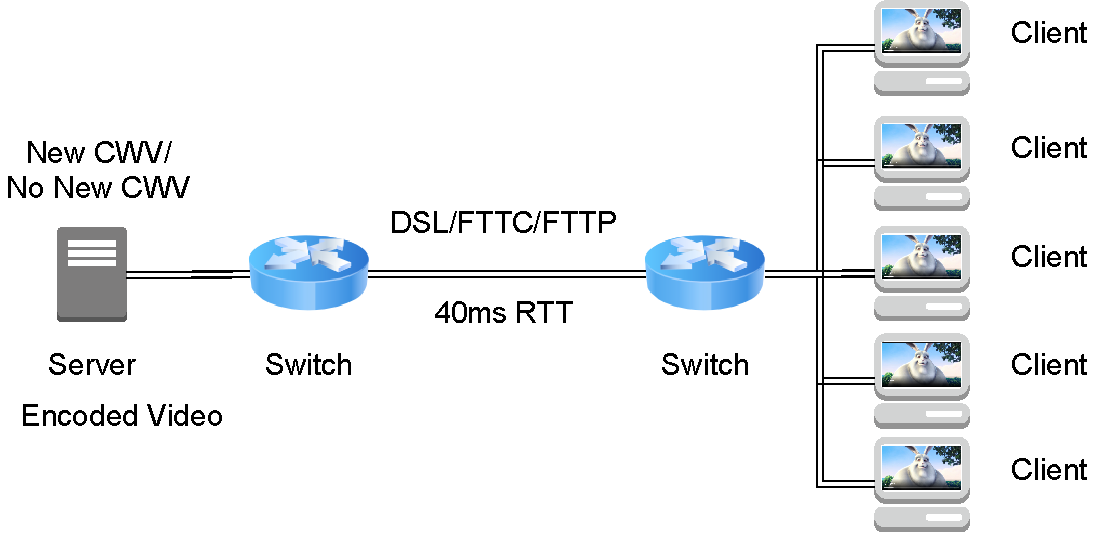
\includegraphics[width=.5\textwidth]{figures/setup.pdf}
  \caption{Experimental Setup}
  \label{fig:experimental-setup}
\end{figure}

Finally, to eliminate noise, we run each \textit{congestion control setting, number of clients, link type} combination 10 times before averaging and reporting results. The dataset presented includes data accumulated over 240 runs (2 algorithms * 3 link types * 4 client variations * 10 repetitions). This accounts for over 2538 minutes or otherwise 42.3 hours of video playtime.

The streamed video is Blender's Big Buck Bunny \cite{online-bbb} (Table \ref{tab:experiments-video} for Details).

Finally, we modify the Linux Kernel's (5.4.0) logger timestamps to be RFC 3339 compliant in order to enable better event tracking. We also provide a ported version of New Congestion Window Validation \cite{rfc7661-2015-fairhurst-new-cwnd-validation} for that kernel. We also modify Reno to log various CWND related events.

From application's point of view, during each run we collect the client's bandwidth estimations. Additionally, to evaluate the video QoE impact we collect information to report average bit-rate, average bit-rate oscillations, and re-buffer ratio as these are standard video metrics directly related to the user's QoE \cite{Spiteri-2019-from-theory-to-practice-sabre, Yin-2015-a-control-theoritic-approach, Dobrian-2013-understanding-the-impact-of-video-quality}.

In addition, we run tcpdump and record all packets on the client and the server, so we can reconstruct the network activity.

% -----------------------
% Previous begining of chapter 4

% To test our hypothesis, we compare two TCP Reno video stream cases, one that does not use New CWV (the current kernel default), and one that does. To measure and quantify the application level performance, we use standard video performance metrics, namely, average bit-rate, average bit-rate oscillation, and rebuffer ratio (Figures \ref{fig:throughput-clients-1} - \ref{fig:throughput-clients-5}). Furthermore, to measure the transport layer impact, we collect throughput measurements as calculated by the receiver's adaptation algorithm (Figures \ref{fig:avg-bitrate} - \ref{fig:rebuffer-ratio}).

% Additionally, we run each of our video scenarios within the environment introduced in \ref{sec:experimental-setup} with 1, 2, 3, and 5 different clients (receivers) that all attempt to request the video at the same time. Finally, we repeat each such instance ten times and then take the average values in order to reduce statistical noise. Following, we split the discussion into two sections: transport and application impact.

% We conduct two sets of measurements. First, we look at the impact of the new CWV algorithm on transport level behaviour, and measure the extent to which adaptive streaming applications using TCP with the new CWV algorithm obtain more consistent throughout estimates. Second, we turn to application level metrics, and measure impact on the selected video bit rate, average bit-rate oscillation, and rebuffer ratio. This allows us to investigate whether the different behaviour in the transport results in different application behaviour.

% \textit{Note:} To present the full picture in with respect to the transport layer we present two different bandwidth measurement values: calculated and advertised throughput. The former is the raw calculation obtained by dividing the chunk size and the transmission time for each received chunk at the client. The latter represents the formal value that the dash.js algorithm uses to make its bitrate selection decision. It is a function of the calculated throughput, then averaged over a sampling period and multiplied by an internal bandwidth safety factor.

% We then look at the average bit-rate (Figures \ref{fig:avg-bitrate-clients-1} - \ref{fig:avg-bitrate-clients-5}), average bit-rate oscillation (Figures \ref{fig:avg-oscillation-clients-1} - \ref{fig:avg-oscillation-clients-5}), and average rebuffer ratios (Figures \ref{fig:rebuffer-ratio-clients-1} - \ref{fig:rebuffer-ratio-clients-5}) for Reno with New CWV enabled and without it. This allows us to investigate whether the different behaviour in the transport results in different application behaviour. We chose to present the aforementioned three properties as they are standard video defining QoE metrics. Average bitrate gives us the overall quality of all rendered video chunks. Average oscillation gives us a metric that shows how frequent quality changes were occurring and what was the amplitude between different switches in terms of bitrate. Finally, rebuffer ratio shows how much of the connection's total time, after the video started playing, was spent waiting for content to be played (rebuffering). The rebuffer ratio is a value between $[0.0 - 1)$, to make reading the results in Figures \ref{fig:rebuffer-ratio-clients-1} to \ref{fig:rebuffer-ratio-clients-1}, we have transformed that value in percentages, meaning that a rebuffer ratio with value of 0.5 would be presented as 50\% and would otherwise suggest that the connection spent half of its time rebuffering.

% Our results confirm our initial hypothesis discussed in Section \ref{sec:newcwv-impact}. In other words, we find that New CWV connections obtain stabler bandwidth estimates compared to Reno. The only exception to this case is the FTTP link, where the difference between Reno and New CWV is not as marginal. We believe this is due to the much higher link capacity combined with the low maximum bandwidth requirement used in the dataset.

% Additionally, we confirm that the more stable bandwidth estimations (Figure \ref{fig:throughput-precise-clients-5} and Figure \ref{fig:throughput-safe-clients-5}) lead to improved QoE. This is evident by the achieved higher bitrate Figure \ref{fig:avg-bitrate-clients-5}, lower Oscillation \ref{fig:avg-oscillation-clients-5}, and lower re-buffer ratio \ref{fig:rebuffer-ratio-clients-5} of New CWV streams compared Reno ones.

% Higher bitrate ratio means that the quality of the rendered frames was higher overall. Lower oscillation means that the players had to switch between different representations less often. This is an important metric, as switching between representations has been reported to be highly noticeable and impeding the user's experience \cite{Spiteri-2016-BOLA,Akhshabi-2012-http-adaptive-players-compete,Huang-2013-downtown-abbey}. Finally, lower rebuffer ratio means that the player spent less time being "frozen" and waiting for new content to be loaded into the buffers before it can play it. The rebuffer ratio is a metric $[0.0 - 1.0)$, which indicates how long of the video "play" duration was spent waiting for more content. For example, a rebuffering ratio of 0.1 would mean that the video was stalled for 10\% of the whole play duration. 

% The throughput estimate that dash.js uses for its bit-rate selection (Figure \ref{fig:throughput-safe-clients-5}) is a function which takes any previous measurements if available and then applies an additional ``network safety'' factor. This is different from the direct throughput value the player calculates by dividing the chunk size and the transmission time (Figure \ref{fig:throughput-precise-clients-5}). We call the former advertised throughput and the latter calculated throughput.

% In figure \ref{fig:throughput-precise-cdf} we see that Reno has more measurements lower than the maximum quality threshold. Consequently, we see that the TCP state of both algorithms allows them to obtain measurements significantly higher than the highest bandwidth requirement for the connection. In practice, any speed measured over the highest media presentation demand is of no significant impact. In other words, regardless of how fast a connection can transmit its 1080p video chunks it will never be able to switch to a higher representation if that is not offered. Therefore, the bandwidth that would otherwise simply allow for faster filling of the client's playback buffer could be otherwise used. This idea could see interesting applications if there existed a congestion control algorithm that could learn the application's bandwidth demands and use that information to clamp the connection's TCP state to not yield any increase in terms of the perceived video quality.   


% We have conducted multiple experiments with  1, 2, 3, and 5 clients for DSL, FTTC, and FTTP representative scenarios. Below we provide a summary of the key findings.

\subsection{Impact on Transport Performance} 
% NewCWV controlled connections have more stable rates, observed by the lower standard deviation in the throughput used by the client algorithm for 10 out of the 12 tested profiles. Additionally, we note that connections using NewCWV consistently measure a lower mean throughput value. In the FTTC case, the mean value reported by NewCWV is closer to the equilibrium value that would be obtained in the case where bandwidth was distributed evenly if all connections were active at the same time. Interestingly, this trend is not carried over the DSL and FTTP scenarios. In fact for the DSL scenarios both algorithms would often report a mean value, higher than the link's available bandwidth. We traced the root cause for this behaviour to be very large congestion window values that allow video chunks to be transmitted in low number of roundtrips, such that the monitoring unit cannot obtain a large enough sample to compute a ``representative'' value.
% \todo{I think this occurs for Reno with DSL, since the off-periods are not always long enough to cause the connection to reset its state. Further investigation is needed.}

New CWV changes how the congestion window (CWND) value in a connection is managed. Thus, since the CWND dictates how many bytes can be in-flight at any given point we expect that the New CWV clients measuring the bandwidth would obtain different values. 

To show this behaviour we collect two distinct but related throughout values - precise and safe, measured by the clients. Both are calculated for each received chunk. The former is simply the received bytes divided by the download time. The latter is a function that the dash.js client uses internally to select the next representation. The function takes the precise measurement, as well as historical data from previous bandwidth probes on that connection and then applies an additional safety factor ($<1.0$) to the measured value. Figures \ref{fig:throughput-clients-1} - \ref{fig:throughput-clients-5} present the cumulative distribution function for all obtained bandwidth measurements.

For the one client case, we obtain results showing that New CWV's faster CWND resumption after idle accounts for these flow being able to obtain higher bandwidth than Reno flows without New CWV. Similar results are also shown in \cite{Nazir-2014-performance-evaluation-congestion-window-validation-dash-newcwv}, confirming that our New CWV port was successful. These results also confirm our initial hypothesis that New CWV controlled flows should be able to get measurements closer to the available link speed, compared to Reno flows without New CWV. 

\begin{figure*}
  \centering
  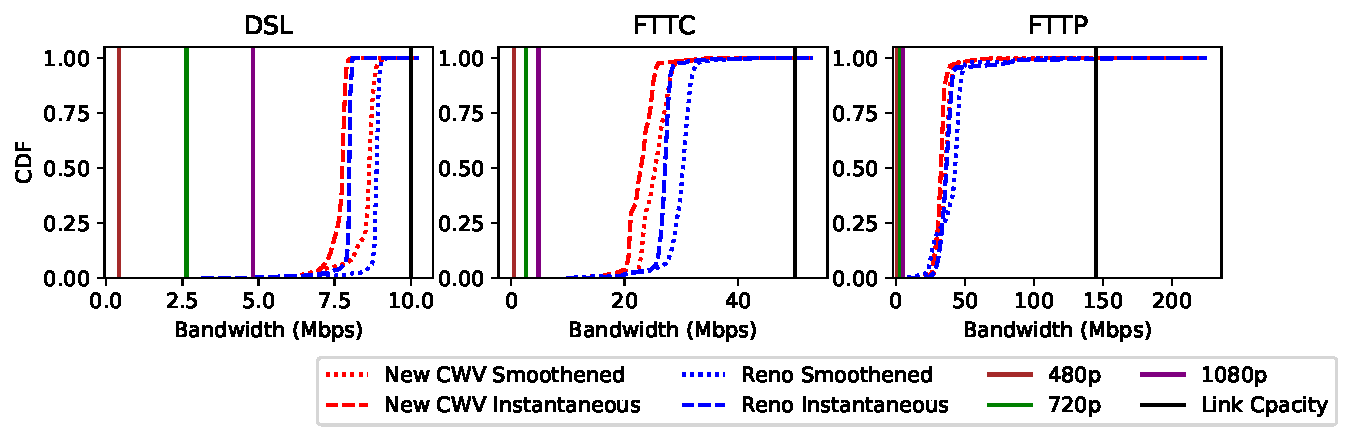
\includegraphics[width=\textwidth]{figures/Throughput_1_clients.pdf}
  \caption{Throughput 1 Client}
  \label{fig:throughput-clients-1}
\end{figure*}

\begin{figure*}
  \centering
  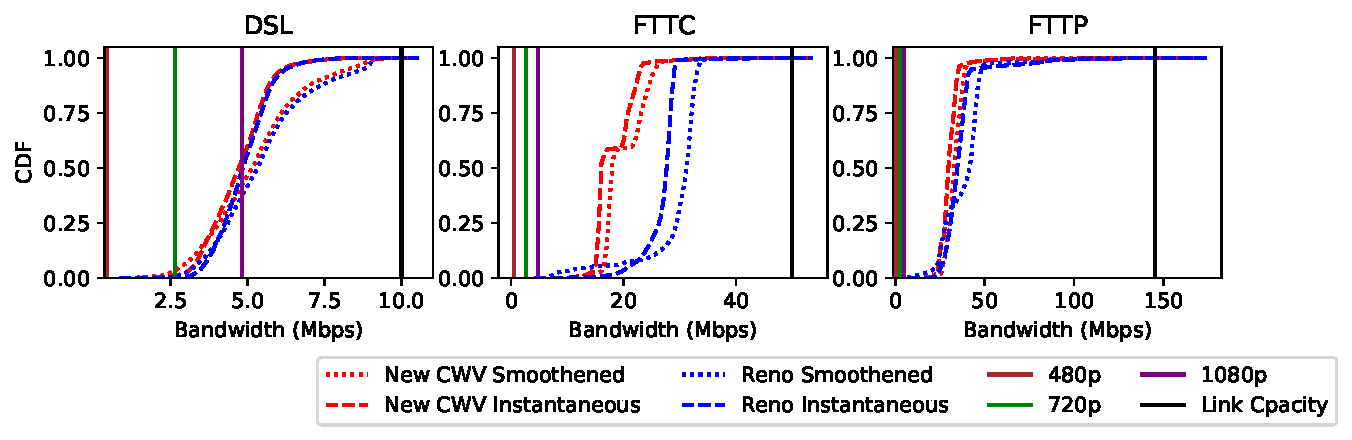
\includegraphics[width=\textwidth]{figures/Throughput_2_clients.pdf}
  \caption{Throughput 2 Clients}
  \label{fig:throughput-clients-2}
\end{figure*}

\begin{figure*}
  \centering
  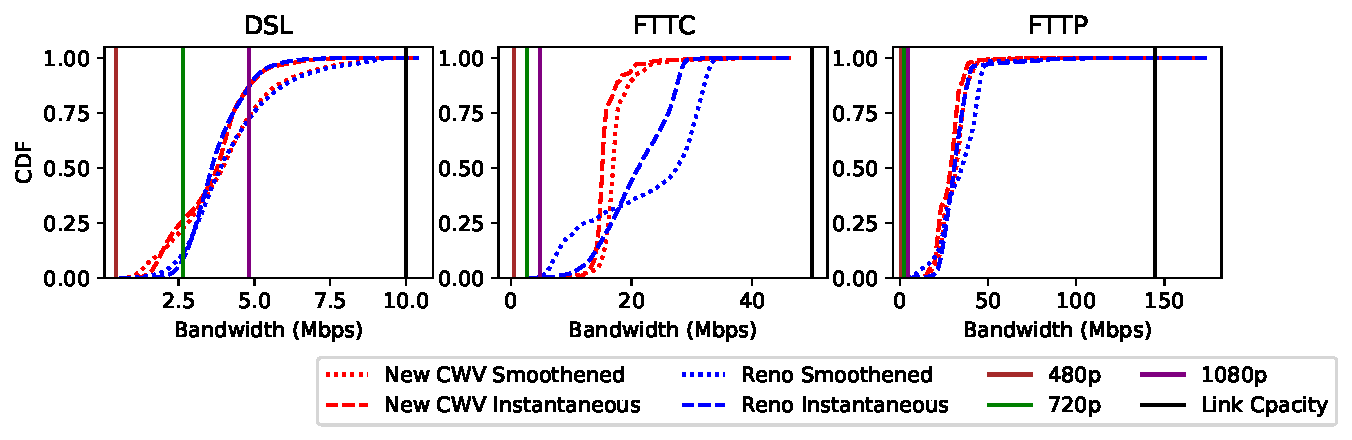
\includegraphics[width=\textwidth]{figures/Throughput_3_clients.pdf}
  \caption{Throughput 3 Clients}
  \label{fig:throughput-clients-3}
\end{figure*}

\begin{figure*}
  \centering
  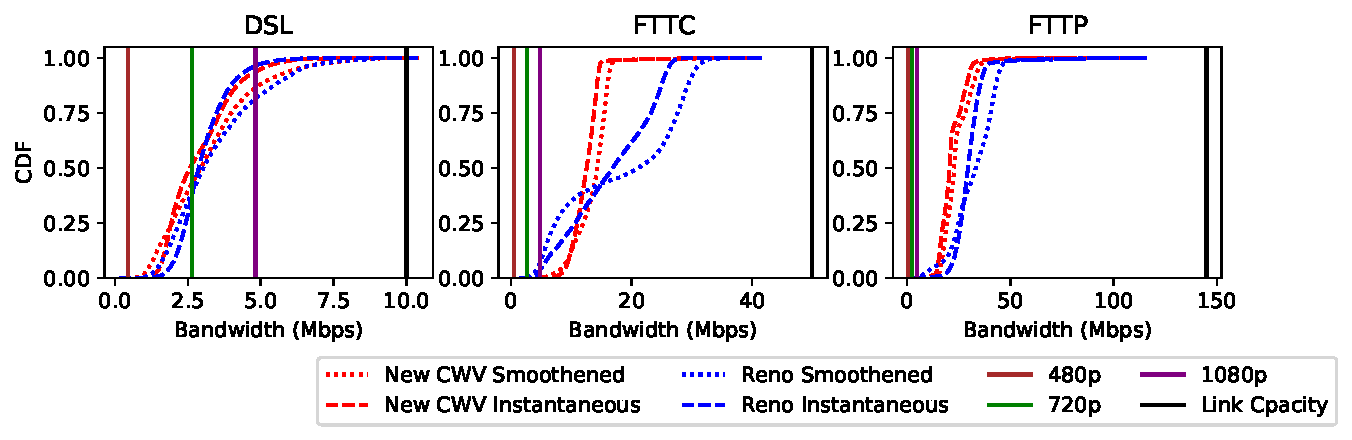
\includegraphics[width=\textwidth]{figures/Throughput_5_clients.pdf}
  \caption{Throughput 5 Clients}
  \label{fig:throughput-clients-5}
\end{figure*}


\subsection{Impact on Video QoE}

To quantify the effect of the different throughput measurements with respect to the achieved QoE, for each run, we calculate average bit-rate, average bit-rate oscillations, and rebuffer ratio.

In Figure \ref{fig:throughput-clients-5}, we see information about the throughput values. On top, we see the different thresholds that dash.js requires in order to select a higher quality. We can see that for both the DSL and FTTC scenarios, New CWV is able to obtain more bandwidth probes over the 1080p limit. Intuitively, this would suggest that in these cases New CWV should obtain higher bitrate. In other words, we expect New CWV connections, to request more segments of the highest quality. We can see that this expectation is confirmed by Figure \ref{fig:avg-bitrate}.

Additionally, from Figure \ref{fig:avg-oscillations} can be observed that New CWV connections not only ramp up to the best available quality faster, but they also have more consistent measurements and better detect that the link has not changed. In contrast, Reno connections would oscillate more between the highest and second-highest quality which would create higher bit-rate oscillation.

Finally, we observe that New CWV connections pace out their idle periods better and avoid synchronizing. This leads to fewer retransmitted packets and overall faster segment transmission. In turn, the client's buffers do not deplete as fast and thus New CWV connections enjoy lower rebuffer ratio, as shown on Figure \ref{fig:rebuffer-ratio}.



\begin{figure*}
  \centering
  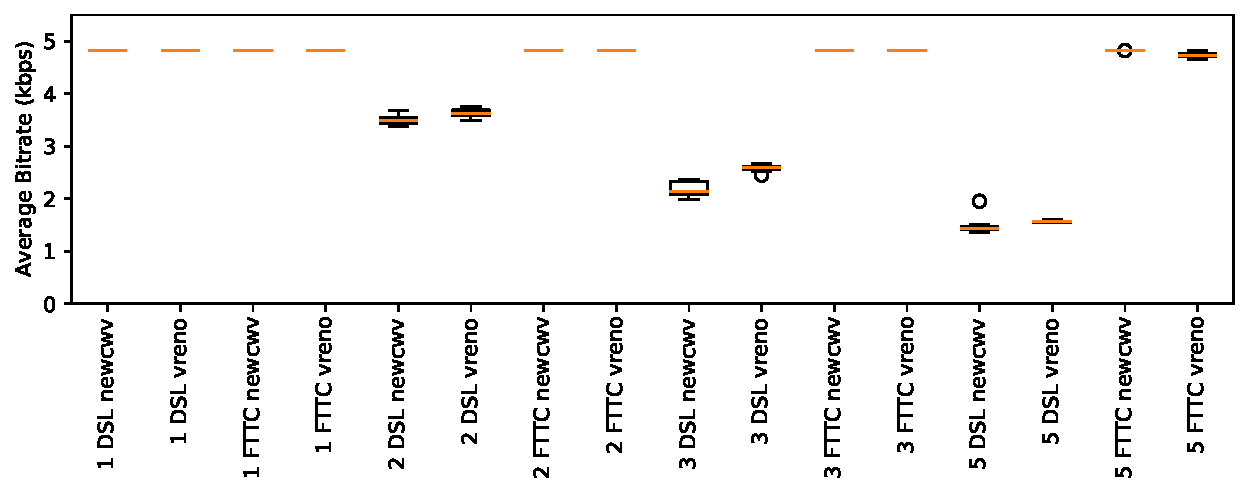
\includegraphics[width=\textwidth]{figures/Average_Bitrate.pdf}
  \caption{Average Bit-rate}
  \label{fig:avg-bitrate}
\end{figure*}


\begin{figure*}
  \centering
  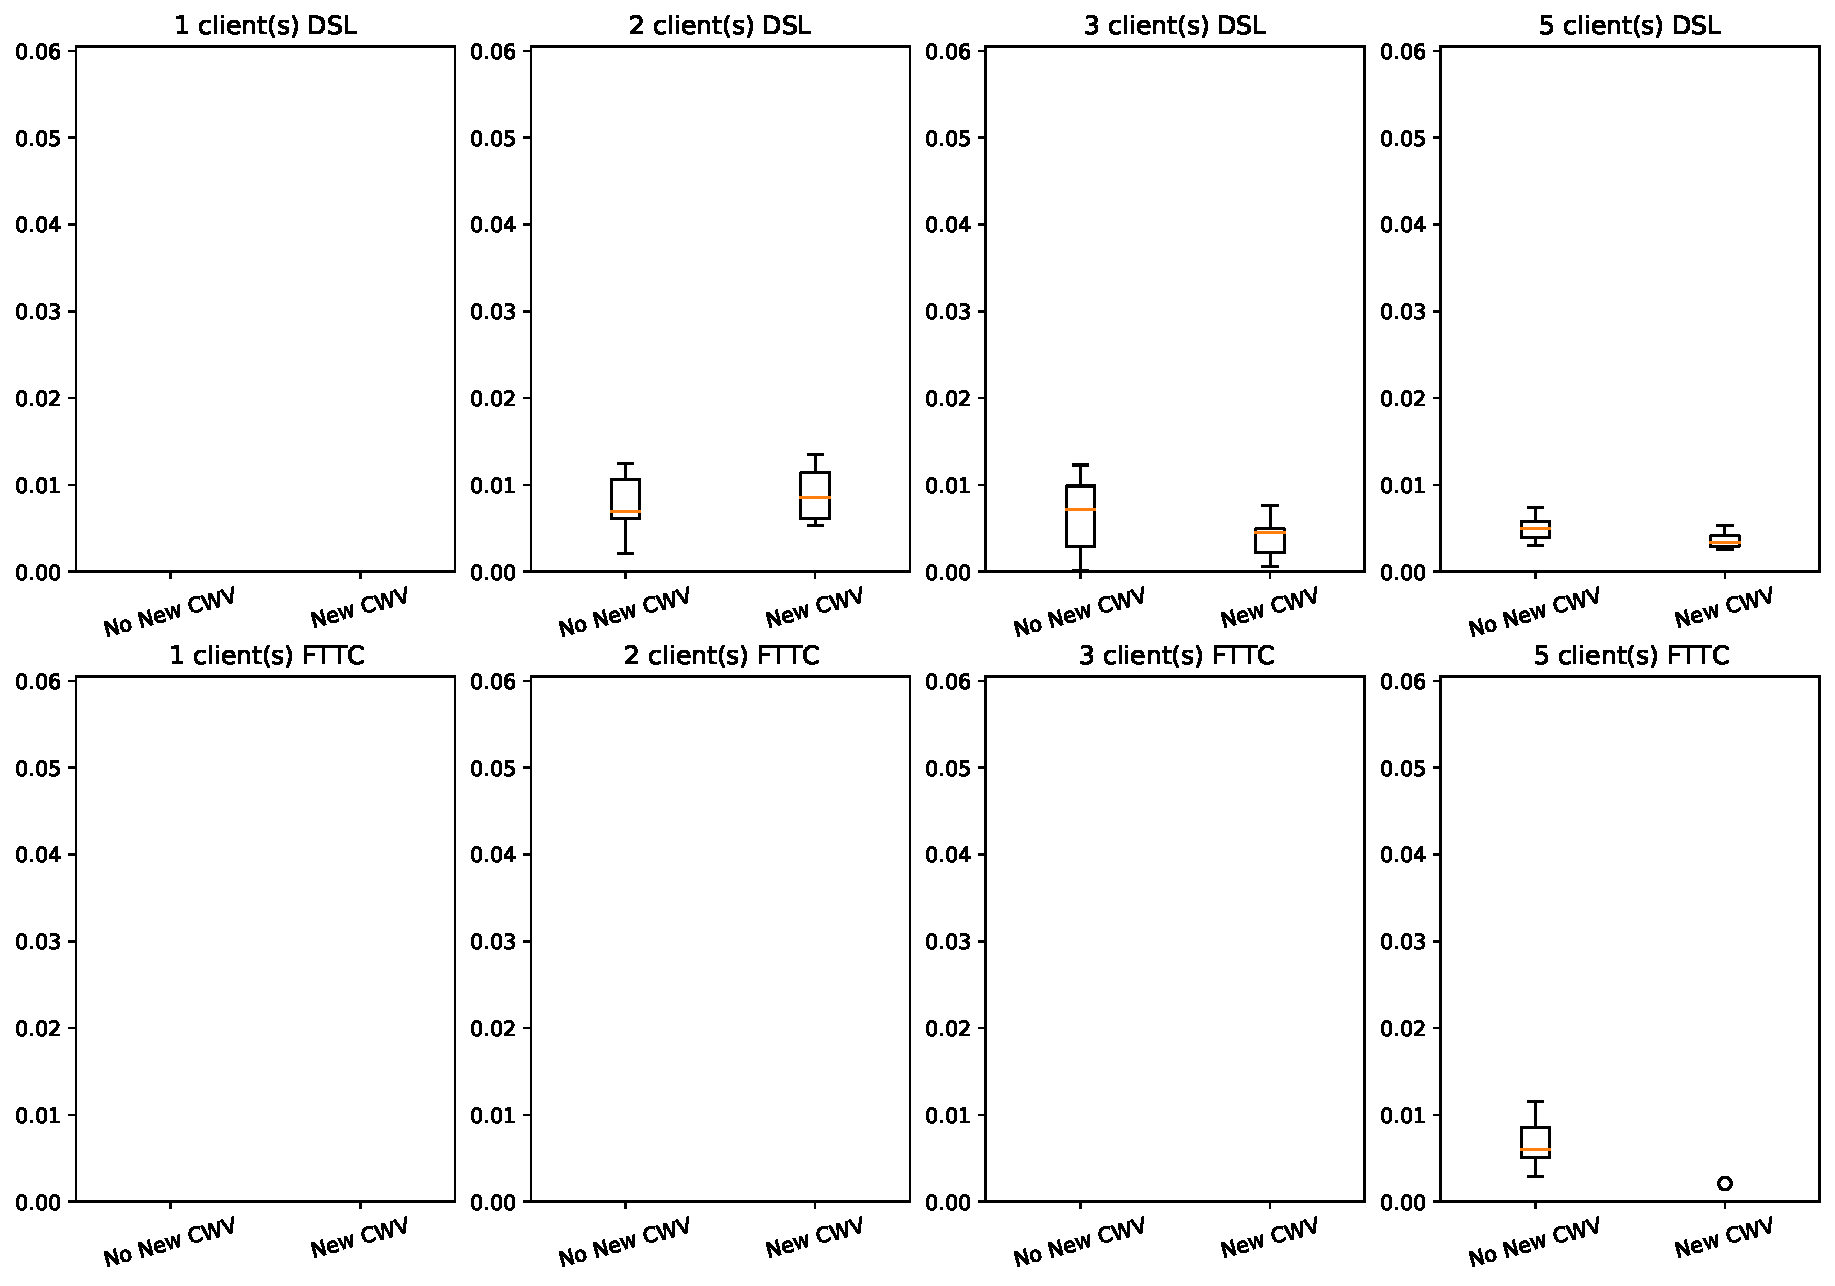
\includegraphics[width=\textwidth]{figures/Average_Oscillations.pdf}
  \caption{Average Bit-rate Oscillations}
  \label{fig:avg-oscillations}
\end{figure*}

\begin{figure*}
  \centering
  \includegraphics[width=\textwidth]{figures/Rebuffer_ratio.pdf}
  \caption{Rebuffer Ratio}
  \label{fig:rebuffer-ratio}
\end{figure*}


% We find that in all but two of the DSL profiles NewCWV connections would obtain a higher average playout bit-rate. Additionally, in all considered scenarios NewCWV showed a mean rebuffering value of under 0.6 seconds for the whole video, while Reno connections without NewCWV would on average enter rebuffering state for over a second in half of the considered scenarios. Peaking at an average of over 20 seconds of rebuffering for the 5 connections over FTTP case. In addition to the lower rebuffering time, we find that NewCWV also achieves comparable or lower mean oscillation in almost all cases.

% Achieving high bitrate with low oscillation are desired properties for any bitrate selection algorithm. In our case, we see that using NewCWV enables the same algorithm to perform better for both of these variables. Previous found high oscillation values to cause poor video QoE \cite{Spiteri-2016-BOLA,Akhshabi-2012-http-adaptive-players-compete,Huang-2013-downtown-abbey}. Finally, the other desired property for any algorithm is the lower rebuffering ratio. Similarly, we see that New CWV enables the same algorithm to perform better in this scenario as well. In other words, the difference of New CWV's CWND resumption after idle is noticeable in the transport layer, enabling the same adaptation algorithm to achieve lower video oscillation and rebuffering with higher bitrate, or otherwise: smoother, higher quality video that does not wait for new content. This directly translates to an increased video QoE. So we conclude that enabling New CWV at the server leads to improved bitrate selection performance and thus higher QoE. This confirms our initial hypothesis.

% \todo{We need to look at the CWND evolution for these connections}

% \todo{verify}
% Maybe true for 1 client

% In terms of the calculated throughput, it should be noted that the New Congestion Window Validation connections consistently report lower throughput estimations compared to their counterpart. We reason this comes from the fact that New Congestion Window Validated connections are less aggressive and do not send as many bursts over the link capacity as the alternative. In turn these episodes where Reno overshoots account for the higher overall reported link bitrate.

% \todo{
% \begin{itemize}
%   \item Should we also look at what happens in the transport layer? I.e., how many idle periods does each connection have on average, how long they are, when they occur, etc.
%   \item Would a mathematical model of what happens after an idle period for Reno and New CWV help? It could find the numbers of additional players where the behaviour between the two could be different.
% \end{itemize}
% }

% As expected, we see that for the FTTP (all links?) link, the New Congestion Window validation simulations yielded a more accurate confidence interval with respect to the available link capacity. 

% In the presented data (f.e., \ref{fig:throughput-precise-FTTP}), we see that both Reno and New Congestion window validation have outliers reporting much higher than the actual link capacity. These outliers are expected. They could happen in the initial requests, when the player does not know anything about the network yet, so it requests the lowest available capacity. In this case,  it requests the 480p encoding which has a bandwidth requirement of 0.44Mbps. The sending capacity of the server at this point is much higher, so the data gets transferred in a single send call. At this point, to obtain an accurate estimation the client would need to keep timestamps with nanosecond precision. This is not the case, so the client could end up significantly overestimating the link capacity. 

% Another thing to note from \ref{fig:throughput-precise-FTTP} is that neither the New Congestion Window Validation nor the Reno connections got close to the real link capacity with their estimations. This is caused by the same phenomenon explained above but on a different scale. In this case, none of the individual video chunks is large enough to reach the sending rate allowed by the channel consistently. In other words, not enough data is being sent over the link, so that the client can get an accurate estimation of the real sending capacity. However, in this particular instance this does not matter, as to support its most demanding encoding the client only needs to know that the link speed is over 12.96 Mbps, which both connection types are able to assess.


% Additionally, Figure \ref{fig:throughput-precise-FTTP} shows one of the effects of the better defined transmission periods for New CWV. On the figure New CWV displays tighter confidence interval on the measured throughput, whereas Reno's inferred values vary more. This behaviour follows directly from Reno's irregular intervals. Varying the transmission time for chunks of same length, naturally translates to less confident bandwidth probes.


% However, we note that at the transport level New CWV results in more predictable sending patterns with better defined boundaries and more granular durations of the periods where the channel is in idle or sending period. For comparison, when not using New CWV these channels are irregular and do not follow a set of patterns. This might suggest that using New CWV, the traffic might be more stable in the presence of cross traffic or when multiple video clients are competing over the same bottleneck link. To demonstrate this, I will conduct a simulation where two clients request video on the DSL link. The results so far show that the client would start requesting the 1080 encoding as it is the highest sustainable for the 10 Mbps provided by DSL. The expected behaviour is that with two competing players both clients should carry on requesting 1080, as the combined bandwidth constraint remains lower than the capacity.


% To evaluate whether the hypothesis that more precise bandwidth estimations could improve streaming stability and to demonstrate to what extent inaccurate measurements contribute to playback instability when using the throughput algorithm we perform an experiment that emulates DSL and FTTC links.
% The link speeds were taken from Ofcom's ``Home Broadband Performance'' and FCC's ``Measuring broadband America'' annual reports (Table \ref{tab:experiments-network}). In all experiments the router queue size was set to the BDP for the connection and the latency was set at 50ms, reported by FCC and observed from our residential link to a Netflix's CDN.



% Experiment plan:
% \begin{itemize}
%     \item New CWV achieves higher precision for obtained bandwidth probes
%     \item If we run an experiment with link speeds close to the required by the player New CWV should stabilise the requesting sooner than non New CWV connections.
%     \item Specific values for link speed and representation should not matter much as this behaviour would occur every time when link capacity is close to the player's request switching threshold. With current technologies this could occur for connections of up to 95 Mbps for 4k HDR video
% \end{itemize}


\begin{table}[]
    \centering
    \begin{tabular}{c|c|c|c}
    \toprule
        Number & Type & Bandwidth (Mbps)  & Latency (ms)  \\
    \midrule
         1 & DSL  & 10  & 40 \\
    \midrule
         2 & FTTC & 50  & 40 \\
    \midrule
         3 & FTTP & 145 & 40 \\
    \bottomrule
    \end{tabular}
    \caption{Experiments' network characteristics}
    \label{tab:experiments-network}
\end{table}

\begin{table}[]
    \centering
    \begin{tabular}{c|c|c}
    \toprule
         Encoding & Bandwidth Required & Segment Duration \\
     \midrule
        480  & 0.44  Mbps & 3 s \\
        720  & 2.64  Mbps & 3 s \\
        1080 & 4.82  Mbps & 3 s \\
        2160 & 12.96 Mbps \textbf{(not in use)} & 3 s \\

    \bottomrule
    \end{tabular}
    \caption{Experiment's Video characteristics}
    \label{tab:experiments-video}
\end{table}

% TODO: Heatmap with all 50 connections

% For all experiments, we stream a 635 second long SDR video from an Nginx server. The client is a Firefox instance using dash.js 3.1.3 using default parameters and "abrThroughput" as its adaptive strategy. We chose to set this strategy as it is one of the three current main ones and would best reflect the impact of accurate link capacity estimations. The video is encoded in 3 second chunks as prior work identified this gives the best trade-off in optimising network load, while minimising video stalls. 

% \begin{itemize}
%     \item CSP Notes
%     \item BBB video
%     \item different link types
% \end{itemize}

% Therefore using properties from the aforementioned scenarios, we propose a set of experiments with network characteristics as shown in Table \ref{tab:experiments-network}. The video is encoded as shown in Table \ref{tab:experiments-video}. The video duration is 635 seconds and we use the default dash.js settings for the throughput algorithm with video buffer length set to 12s (default). This means that after the client has buffered 12 seconds of video, we expect to see long on-off periods equal to the segment duration (3 seconds). As discussed earlier, the specific details of the link capacity and encodings do not matter but we have chosen these values as the link capacityies resemble DSL (experiment \#1) and FTTC (experiment \#2) links. The video encoding rates are taken from YouTube's reference values and the connection RTT is set to a value representative of reported latency on DSL links to a measurement site in US.

% We choose not to introduce cross traffic and change the link speed in order clear the observed results from any noise that could be introduces by either of these phenomena. Moreover, the scenario would be representative of a single user requesting video on a DSL connection.


% \subsection{Setup}

% \idea{
% \begin{itemize}
%     \item New CWV verification
%     \item Kernels
%     \item Adaptation algorithm
%     \item Network setup
% \end{itemize}
% }

% We would like to assess the effect that slow-start CWND spikes have with respect to the video's application performance. To demonstrate that, we compared Reno and New CWV as an example of two protocols, one affected by the issue and the other one non-affected by it.

% To carry that study, we wrote New CWV for Linux kernel 5.4.x series, as the previous implementation was for 3.8.x. Then we verified that our implementation is correct by validating it against the RFC. With that setup and exposing additional state from the DASH.JS adaptive algorithm, we were able to collect information about the players' throughput estimates. We then tested both algorithms for cases where the network capacity is: (i) close the required capacity by one of the video representations, (ii) between two different video representation requirements, and finally (iii) much more than the highest representation requirement.

% In cases where the link capacity is close to one of the representations, we expect it to either produce false positives or false negatives. Depending on whether the link capacity is under or over the required by the video representation. For cases that the link capacity is between two representation values, we do not expect to see significant difference, as a wrong bandwidth probe is likely to keep requesting the supported rate. Finally, for cases where the link capacity is much more than that required by the highest representation, we would again expect to see no difference as likely each video transfer would never exit the slow-start phase.

% Furthermore, as we expect New CWV would to produce different results compared to Reno in only one of those three cases the benefits of using New CWV would be proportional to how likely that issue is to occur in a real network scenario. According to the recommended encoding rates by YouTube \url{https://support.google.com/youtube/answer/1722171?hl=en#zippy=%2Cbitrate%2Cresolution-and-aspect-ratio},
% this issue would affect links with capacity of up to 24 or 30 Mbps for SDR and HDR for Full HD videos and up to 68 to 85 Mbps for Utra HD videos. However, most videos would be offered in up to 1080p quality as the users would not notice any difference than higher video, or the encoders did not produce it, or the network cannot support it (EU asking Netflix and Amazon to reduce their video quality because of COVID-19).


% We ported New CWV for linux kernel 5.4.x series. To verify that the port was successful, we compared the performance of the ported New CWV and the authors' New CWV implementation for kernel 3.18.2. In both cases, we emulated the network conditions and dataset from \cite{Nazir-2014-performance-evaluation-congestion-window-validation-dash}. We then streamed that content on a Firefox client using dash.js's (v 3.1.3) throughput algorithm and we used nginx to serve the content.

\section{Discussion}

Figures \ref{fig:throughput-precise-clients-1} - \ref{fig:throughput-safe-clients-5} show that Reno reports more data points with throughput value lower than the highest bandwidth requirement. Consequently, both algorithms have a high amount of data points over the highest bandwidth requirement. In practice, any speed measured over that requirement is of no significant impact. Higher values only allow the client's playback buffer to fill faster but would not enable a switch to a higher representation, since such is simply not being offered. Thus, any video connection would see limited gains beyond measuring any values beyond the connection's maximum bandwidth demand. This would mean that connections could be clamped at a given rate and the rest of the ``spare'' bandwidth could be used-up by other traffic. This idea could see interesting applications if there existed a congestion control algorithm that could learn the application's bandwidth demands and use that information to limit the connection's congestion window and not allow it to grow beyond a set value. The implications might be various from more video connections being able to reach their demands to non-video traffic performing better since video does not need to be aggressive beyond a given point. However, implementing such an algorithm would be hard since it raises many unknowns about how such an algorithm would react to lost packets and when it would slow down such that it is not beaten by other more aggressive traffic, would a standard AIMD or CUBIC function for controlling CWND growth suffice or would there be other alternatives, etc.

% To verify whether New CWV's more accurate bandwidth estimations could improve playback stability, we would run three scenarios. Two with network link speed close to a representation requirement, and another sufficiently higher than a selected representation requirement.

% In other words, if we have requirement of $R$ bits per second to support given representation $X$ where $X$ is not the lowest representation in the set. The current reference player behaviour is to start requesting $X$, as soon its average bandwidth estimate becomes $R/C_{bsf}$, where $C_{bsf}$ is the bandwidth safety factor (default 0.9). In this scenario, the more accurate bandwidth probes that New CWV might produce would mean that the player would start requesting $X$, sooner than it would if the connection was not using New CWV.

% In specific, assume a video is encoded as shown in Table \ref{tab:video-requirements}. Then the average bandwidth estimate that the player would need to start requesting the 1080p representation would be 12.32 Mbps. Therefore, if we set the link speed at 13.55 ($12.32 + 10\% * 12.32$) we would expect the New CWV connection to attempt switching to the higher rate, whereas the non New CWV connection would keep requesting the 720p. Furthermore, for link speed of 14.78 ($12.32 + 20\%*12.32$), we would expect the New CWV to stably request the 1080p, whereas the non New CWV connection would be requesting a mix of 720 and 1080, depending on whether the average bandwidth probe exceeds 12.32 Mbps or not. Similarly, for link speed of 16.01 ($12.32 + 30\% 12.32$), we would expect both the New CWV enabled and the New CWV disabled connections to steadily request the higher 1080p representation. 

% In this scenario, the values for the link speed and encoding representations are not important. Rather, they show a pattern relating to any scenario with similar $X$ and $T$ values. In other words, while we use a specific example to demonstrate a problem here, it may arise for any connection with link capacity of up to 100 Mbps. \\(\url{https://support.google.com/youtube/answer/1722171?hl=en#zippy=%2Cbitrate%2Cresolution-and-aspect-ratio})

% \begin{itemize}
%     \item New Transport ideas
%     \item This chapter comes to the conclusion that while New CWV might be able to report more accurate results, in the scenarios for VoD streaming that we have today, they do not make a difference.
%     \item However, if there was a proposal that promised an even more accurate bandwidth reporting, then the application could use that to better determine if representation $R$ is sustainable.
% \end{itemize}

% Prior work evaluated New CWV against TCP Reno using a Linux kernel 3.14 implementation. Since then the Linux's Reno implementation has been a subject to both further optimisations (i.e., adoption of newer proposals) and API changes.

% A comparison of the current Reno implementation with a decade old New CWV would be unfair and the observed results might be due to improvements in Reno. To overcome this issue we provide a New CWV port for the most modern long term supported kernel of Linux (5.4). To verify that the port is success full and represent behaves as expected, we created 7 test-cases taken from RFC7661 and verify that our implementation behaves as documented.

% \section{Evaluation Metrics}

% % One aspect that was not considered with New CWV's proposal was its impact on the application layer. As discussed in chapter \ref{sec:background} the HTTP video streaming community have converged to a set of metrics that are considered most impactful for a stream's quality of experience. We believe that the lack of adoption of New CWV can be explained by a lack of increase in any of these metrics. \textbf{Claim: }In other words, standard Reno and New CWV should produce results of non significant difference.

% % To verify this claim, we compared the application layer results of Reno and New CWV. We used two network-data-set pairs for this experiment. For the first, we re-used the setup in \cite{Nazir-2014-performance-evaluation-congestion-window-validation-dash}, for the second, we used video bit-rate encodings recommended by YouTube \cite{} and represnetative network trace that we picked from \textit{``Measuring Broadband America''} \cite{}.

% % Rk  , Bk and Ck represents the video bitrate, buffer occupancy and bandwidth capacity for chunk K respectively

% \subsection{Client's throughput probes}

% Since we assess that throughput algorithms that use New CWV as a transport should obtain more consistent results that closer match the effective available bandwidth, we collect all throughput samples reported by the client.


% Then, to evaluate the application-level performance we use the following metrics, used by both industry and research.

% \subsection{Average Bit-rate}

% The average video bit-rate is the sum of the bit-rates of all played-out chunks divided by their number. However, measuring bit-rate alone is not enough to estimate the QoE. For this reason additional metrics, described below are also considered. In addition, bit-rate improvement is not always proportional to an increase in QoE. For example a video representation changing from 1 to 2 Mbps, will achieve higher QoE than another stream changing from 10 to 11 Mbps, even though the bit-rate increase was the same \cite{Spiteri-2019-from-theory-to-practice-sabre}.

% \begin{equation*} \frac {1}{k}\sum _{k=1}^{K}q(R_{k}) \end{equation*}

% \subsection{Average Bit-rate oscillation}

% Mok et al show that frequent changes in the quality of the requested video is decremental to user's QoE \cite{Mok-2011-inferring-qoe}. The effective oscillation index can be computed using the average bit-rate oscillation formula. It measures the depth of the representation changes in the playout process. Proposals trying to optimise for this criterion exist \cite{Mok-2012-qdash, Huang-2012-confused-timid-qoe}.

% \begin{equation*} \frac {1}{K-1}\sum _{k=1}^{K-1}|q(R_{k+1})-q(R_{k)}| \end{equation*}

% \subsection{Startup delay \& Rebuffer Ratio} 

% Startup delay is the observed latency from when a video play request has been issued (e.g., user clicks the play button) to the first video frame starting to play-out. Rebuffer events occur when the video has no available buffered content and has to stop playing in order to fill in the buffers. This occurs when the media download time is higher than the playout buffer level. Research has shown that high startup delays or long rebuffer events could lead to users abandoning the video or watching less of it cite \cite{Krishnan-2012-video-stream-quality-impacts}.

% \begin{equation*} \sum _{k=1}^{K}\left ({\frac {d_{k}(R_{k})}{C_{k}}-B_{k}}\right)_{+} \end{equation*}

% \subsection{Metrics Summary}

% Striving for a single QoE metric has been an active research area. \cite{Yin-2015-a-control-theoritic-approach} aims to come up with a formula that uses the four metrics above, while \cite{Balachandran-2012-a-quest-for-internet-qoe} attempt to solve the problem by applying machine learning. However, no single such equation has been widely accepted. Instead, all work aiming to produce such equation relies on the same four metrics described above. 
% \cite{Dobrian-2013-understanding-the-impact-of-video-quality} classifies them as the industry standard. 

% \section{Evaluation}

% In order to obtain the metrics introduced in the previous chapter, we would need to stream a video over a period of time. During the play-out, results of the reported throughput would be collected.

% As an input for the experiment we would need to know how the network looks like, i.e.,
% \begin{enumerate}
%     \item what is the available bandwidth for the link
%     \item what is the connection RTT
%     \item Does the bandwidth change?
% \end{enumerate}

% I think here we can take a look at three main cases with respect to the available bandwidth:
% \begin{enumerate}
%     \item Link capacity is much more than the required bandwidth
%     \item Link capacity is close to one of the bandwidths required by the representation
%     \item Link capacity is between two different representation requirements.
% \end{enumerate}

% There was a study 2014 measuring Youtube's average RTT to be around 70, while netflix's 250. Stephen measured RTT to netflix of 50 yesterday so a value 50-70 ms is ``safe''.

% I expect New CWV controlled application to report results closer to the link capacity at all times. However, due to the current practices in modern DASH algorithms, that may not necessarily result in a higher quality as they tend to apply a safety factor on the obtained bandwidth result.

% To show how New CWV affects the application layer using the metrics explained above, we provide results from two network scenarios. The first, explained below re-uses the dataset and network properties as described in the original paper. The second one uses a more modern dataset, taken from youtube's video encoding recommendations and network traces derived from FCC's measuring broadband America 2018 study.

% This way we can verify how impactful New CWV was at the time of its introduction and we will be able to track if the same trend preserved over the years. In other words, we would verify whether the need of CWV is still relevant after almost a decade of evolution in both the network infrastructure and the transport protocols.


% Video: BigBuckBunny \\
% Segment Duration: 2s \\
% Video encodings: 0.2, 0.25, 0.3, 0.4, 0.5, 0.6, 0.7 Mbps \\

% Network: 200ms RTT, 1Mbps link capacity

% \subsection{Scenario 2}

% Video: BigBuckBunny \\
% Segment Duration: 3s \\
% Video encodings: 1.5, 4, 7.5, 12 Mbps \\

% Network: Dynamic taken from FCC

% \idea{
% \begin{itemize}
%     \item Verify New CWV's application impact
% \end{itemize}
% }

% We now show what application layer performance New CWV would have had compared to Reno if the original dataset and link properties were used with a modern throughput-based algorithm. 

% \begin{figure*}
%     \centering
%     \includegraphics[width=\textwidth]{figures/New CWV/cwnd_kernel.pdf}
%     \caption{Congestion Window Progression}
%     \label{fig:cwnd-reno-comparison}
% \end{figure*}

% Figure \ref{fig:cwnd-reno-comparison} compares the CWND evolution over time for Reno and New CWV. Since New CWV is based on Reno, we can see that during network-limited transfers they behave similar to one another (e.g., 100-400 second mark). Additionally New CWV does not grow its CWND to artificially large values during application-limited transfer. On the other hand, we can see Reno doing this after the 500th second mark. In other words, New CWV manages to keep the CWV more stable compared to Reno, by not overshooting its CWND value. In turn, this results in more consistent measurements at the client.

% \begin{figure*}
%     \centering
%     \includegraphics[width=\textwidth]{figures/New CWV/app_metrics.pdf}
%     \caption{Application Level Metrics}
%     \label{fig:app_metrics}
% \end{figure*}

% After seing that New CWV manages to shape the CWND of application-limited transfers to behave as "standard" TCP congestion window, we take a look at the application-layer performance. Figure \ref{fig:app_metrics} shows the start-up delay, average bit-rate, and bit-rate oscillation achieved during our simulations. The last bar-pair depicts the average values across all simulations. In Section \ref{sec:background} we covered the little New CWV adoption. The results, shown in Figure \ref{fig:app_metrics} could be one reason for this. Even though New CWV does provide lower start-up delay and bit-rate oscillation and higher average throughput, the demonstrated gain is not really statistically significant.


% \section{Future Work}

% \idea{New CWV does not help application layer throughput measuring functions to achieve higher precision. }

% New CWV does not show significantly different results from Reno. One way of improving this, would be by achieving lower average bit-rate oscillation. One way this could be achieved is by introducing TCP that leverages a steadier congestion window. This way, client algorithms measuring the throughput will be able to obtain rates that closer match the current network's capacity. In turn, this would lead to more consistent throughput measurements which are therefore less likely to request a rate that does not fully utilise the available bandwidth.

% While New CWV alone does not improve application's performance metrics or user's QoE. It has the correct approach in helping towards a possible improvement in that area. For example, if all results obtained by the application did not need to be validated and normalised, it could mean that applications are able to detect changes in the network more reliably and to react faster.

% The details

% Describe results carefully:
%  - clearly state assumptions
%  - give enough information to allow the reader to recreate the results
%  - ensure results are representative; statistically meaningful, etc.
%  - don't overstate results
%  - equally, don't understate them: consider the broader implications



%==================================================================================================
\section{Related Work}


% This should come near the end, and focusing on discussing how your work
% relates to that of others. Any relevant related work should have been
% cited already, so this is not a list of related work, it's a discussion
% of how that work relates.
%
% Why not put related work after the introduction? 1) because describing
% alternative approaches gets between the reader and your idea; and 2)
% because the reader knows nothing about the problem yet, so your
% (carefully trimmed) description of various technical trade-offs is
% absolutely incomprehensible.
% 
% When writing the related work:
%  - Give credit to others where it's due; this doesn't diminish the
%    credit you get from your paper. 
%  - Acknowledge weaknesses in your approach.
%  - Ensure related work is accurate and up-to-date



%==================================================================================================
\section{Conclusions}



%==================================================================================================
\section{Acknowledgements}

% Acknowledge funding sources.

%==================================================================================================
% Set the bibliography style. Choose one of the following, depending on the
% document class being used:
%
%   \bibliographystyle{abbrv}                 When using article class
%   \bibliographystyle{IEEEtran}              When using IEEE style
%   \bibliographystyle{ACM-Reference-Format}  When using ACM style

\bibliographystyle{ACM-Reference-Format}

% Load the bibliography file(s) for this paper:
\bibliography{paper}

%==================================================================================================
% The following information gets written into the PDF file information:
\ifpdf
  \pdfinfo{
    /Title        (...)
    /Author       (...)
    /Subject      (...)
    /Keywords     (..., ..., ...)
    /CreationDate (D:20150827110616Z)
    /ModDate      (D:20150827110616Z)
    /Creator      (LaTeX)
    /Producer     (pdfTeX)
  }
  % Suppress unnecessary metadata, to ensure the PDF generated by pdflatex is
  % identical each time it is built. This needs pdfTeX 3.14159265-2.6-1.40.17
  % or later.
  \ifdefined\pdftrailerid
    \pdftrailerid{}
    \pdfsuppressptexinfo=15
  \fi
\fi

\clearpage
\appendix{APPENDIX: Extra items}

\onecolumn
\begin{longtable}{{l|l|l|l|l|l|l}}
  
  % \begin{tabular}{l|l|l|l|l|l|l}
  \toprule
    Metric & Link & Clients & Algorithm & Mean & Standard Deviation & 99th Percentile \\
  \midrule
  Rebuffer Ratio & DSL & 1 & newcwv & 0.000 & 0.000 & 0.001 \\
  Rebuffer Ratio & DSL & 1 & vreno & 0.000 & 0.000 & 0.000 \\
  \midrule
  Rebuffer Ratio & DSL & 2 & newcwv & 0.000 & 0.000 & 0.001 \\
  Rebuffer Ratio & DSL & 2 & vreno & 0.001 & 0.002 & 0.006 \\
  \midrule
  Rebuffer Ratio & DSL & 3 & newcwv & 0.001 & 0.001 & 0.003 \\
  Rebuffer Ratio & DSL & 3 & vreno & 0.002 & 0.004 & 0.017 \\
  \midrule
  Rebuffer Ratio & DSL & 5 & newcwv & 0.001 & 0.002 & 0.007 \\
  Rebuffer Ratio & DSL & 5 & vreno & 0.012 & 0.015 & 0.048 \\
  \midrule
  Rebuffer Ratio & FTTC & 1 & newcwv & 0.000 & 0.000 & 0.000 \\
  Rebuffer Ratio & FTTC & 1 & vreno & 0.000 & 0.000 & 0.000 \\
  \midrule
  Rebuffer Ratio & FTTC & 2 & newcwv & 0.000 & 0.001 & 0.003 \\
  Rebuffer Ratio & FTTC & 2 & vreno & 0.000 & 0.001 & 0.002 \\
  \midrule
  Rebuffer Ratio & FTTC & 3 & newcwv & 0.000 & 0.000 & 0.002 \\
  Rebuffer Ratio & FTTC & 3 & vreno & 0.003 & 0.004 & 0.016 \\
  \midrule
  Rebuffer Ratio & FTTC & 5 & newcwv & 0.001 & 0.002 & 0.006 \\
  Rebuffer Ratio & FTTC & 5 & vreno & 0.025 & 0.036 & 0.115 \\
  \midrule
  Rebuffer Ratio & FTTP & 1 & newcwv & 0.000 & 0.000 & 0.000 \\
  Rebuffer Ratio & FTTP & 1 & vreno & 0.000 & 0.000 & 0.000 \\
  \midrule
  Rebuffer Ratio & FTTP & 2 & newcwv & 0.000 & 0.000 & 0.000 \\
  Rebuffer Ratio & FTTP & 2 & vreno & 0.000 & 0.001 & 0.004 \\
  \midrule
  Rebuffer Ratio & FTTP & 3 & newcwv & 0.000 & 0.001 & 0.005 \\
  Rebuffer Ratio & FTTP & 3 & vreno & 0.003 & 0.004 & 0.015 \\
  \midrule
  Rebuffer Ratio & FTTP & 5 & newcwv & 0.001 & 0.002 & 0.006 \\
  Rebuffer Ratio & FTTP & 5 & vreno & 0.000 & 0.001 & 0.004 \\
  \midrule
  Average Bitrate & DSL & 1 & newcwv & 4.823 & 0.004 & 4.825 \\
  Average Bitrate & DSL & 1 & vreno & 4.825 & 0.000 & 4.825 \\
  \midrule
  Average Bitrate & DSL & 2 & newcwv & 3.721 & 0.011 & 3.737 \\
  Average Bitrate & DSL & 2 & vreno & 3.731 & 0.019 & 3.752 \\
  \midrule
  Average Bitrate & DSL & 3 & newcwv & 4.049 & 0.133 & 4.100 \\
  Average Bitrate & DSL & 3 & vreno & 4.025 & 0.076 & 4.106 \\
  \midrule
  Average Bitrate & DSL & 5 & newcwv & 4.247 & 0.193 & 4.390 \\
  Average Bitrate & DSL & 5 & vreno & 3.975 & 0.023 & 4.023 \\
  \midrule
  Average Bitrate & FTTC & 1 & newcwv & 4.825 & 0.000 & 4.825 \\
  Average Bitrate & FTTC & 1 & vreno & 4.825 & 0.000 & 4.825 \\
  \midrule
  Average Bitrate & FTTC & 2 & newcwv & 4.823 & 0.005 & 4.825 \\
  Average Bitrate & FTTC & 2 & vreno & 4.802 & 0.026 & 4.825 \\
  \midrule
  Average Bitrate & FTTC & 3 & newcwv & 4.823 & 0.003 & 4.825 \\
  Average Bitrate & FTTC & 3 & vreno & 4.673 & 0.042 & 4.766 \\
  \midrule
  Average Bitrate & FTTC & 5 & newcwv & 4.824 & 0.004 & 4.825 \\
  Average Bitrate & FTTC & 5 & vreno & 4.334 & 0.039 & 4.391 \\
  \midrule
  Average Bitrate & FTTP & 1 & newcwv & 4.825 & 0.000 & 4.825 \\
  Average Bitrate & FTTP & 1 & vreno & 4.825 & 0.000 & 4.825 \\
  \midrule
  Average Bitrate & FTTP & 2 & newcwv & 4.825 & 0.000 & 4.825 \\
  Average Bitrate & FTTP & 2 & vreno & 4.810 & 0.017 & 4.825 \\
  \midrule
  Average Bitrate & FTTP & 3 & newcwv & 4.824 & 0.003 & 4.825 \\
  Average Bitrate & FTTP & 3 & vreno & 4.655 & 0.051 & 4.739 \\
  \midrule
  Average Bitrate & FTTP & 5 & newcwv & 4.820 & 0.006 & 4.825 \\
  Average Bitrate & FTTP & 5 & vreno & 4.820 & 0.007 & 4.825 \\
  \midrule
  Average Oscillations & DSL & 1 & newcwv & 0.002 & 0.004 & 0.010 \\
  Average Oscillations & DSL & 1 & vreno & 0.000 & 0.000 & 0.000 \\
  \midrule
  Average Oscillations & DSL & 2 & newcwv & 0.004 & 0.001 & 0.005 \\
  Average Oscillations & DSL & 2 & vreno & 0.004 & 0.003 & 0.010 \\
  \midrule
  Average Oscillations & DSL & 3 & newcwv & 0.002 & 0.001 & 0.003 \\
  Average Oscillations & DSL & 3 & vreno & 0.003 & 0.002 & 0.007 \\
  \midrule
  Average Oscillations & DSL & 5 & newcwv & 0.001 & 0.001 & 0.004 \\
  Average Oscillations & DSL & 5 & vreno & 0.010 & 0.003 & 0.016 \\
  \midrule
  Average Oscillations & FTTC & 1 & newcwv & 0.000 & 0.000 & 0.000 \\
  Average Oscillations & FTTC & 1 & vreno & 0.000 & 0.000 & 0.000 \\
  \midrule
  Average Oscillations & FTTC & 2 & newcwv & 0.001 & 0.002 & 0.005 \\
  Average Oscillations & FTTC & 2 & vreno & 0.003 & 0.004 & 0.010 \\
  \midrule
  Average Oscillations & FTTC & 3 & newcwv & 0.001 & 0.001 & 0.003 \\
  Average Oscillations & FTTC & 3 & vreno & 0.011 & 0.005 & 0.020 \\
  \midrule
  Average Oscillations & FTTC & 5 & newcwv & 0.000 & 0.000 & 0.001 \\
  Average Oscillations & FTTC & 5 & vreno & 0.012 & 0.004 & 0.017 \\
  \midrule
  Average Oscillations & FTTP & 1 & newcwv & 0.000 & 0.000 & 0.000 \\
  Average Oscillations & FTTP & 1 & vreno & 0.000 & 0.000 & 0.000 \\
  \midrule
  Average Oscillations & FTTP & 2 & newcwv & 0.000 & 0.000 & 0.000 \\
  Average Oscillations & FTTP & 2 & vreno & 0.003 & 0.004 & 0.010 \\
  \midrule
  Average Oscillations & FTTP & 3 & newcwv & 0.000 & 0.001 & 0.003 \\
  Average Oscillations & FTTP & 3 & vreno & 0.008 & 0.004 & 0.013 \\
  \midrule
  Average Oscillations & FTTP & 5 & newcwv & 0.001 & 0.002 & 0.005 \\
  Average Oscillations & FTTP & 5 & vreno & 0.002 & 0.002 & 0.005 \\
  \midrule
  Throughput Precise & DSL & 1 & newcwv & 8.168 & 0.777 & 8.994 \\
  Throughput Precise & DSL & 1 & vreno & 8.605 & 0.507 & 9.077 \\
  \midrule
  Throughput Precise & DSL & 2 & newcwv & 12.110 & 8.626 & 34.046 \\
  Throughput Precise & DSL & 2 & vreno & 12.953 & 9.343 & 34.744 \\
  \midrule
  Throughput Precise & DSL & 3 & newcwv & 11.617 & 14.741 & 24.714 \\
  Throughput Precise & DSL & 3 & vreno & 13.273 & 8.702 & 32.873 \\
  \midrule
  Throughput Precise & DSL & 5 & newcwv & 9.733 & 3.871 & 16.115 \\
  Throughput Precise & DSL & 5 & vreno & 13.006 & 30.516 & 32.069 \\
  \midrule
  Throughput Precise & FTTC & 1 & newcwv & 23.829 & 3.655 & 35.051 \\
  Throughput Precise & FTTC & 1 & vreno & 28.491 & 3.790 & 37.613 \\
  \midrule
  Throughput Precise & FTTC & 2 & newcwv & 14.585 & 4.745 & 35.859 \\
  Throughput Precise & FTTC & 2 & vreno & 15.270 & 6.696 & 36.696 \\
  \midrule
  Throughput Precise & FTTC & 3 & newcwv & 12.323 & 3.364 & 27.362 \\
  Throughput Precise & FTTC & 3 & vreno & 15.742 & 7.741 & 36.413 \\
  \midrule
  Throughput Precise & FTTC & 5 & newcwv & 10.266 & 4.681 & 16.057 \\
  Throughput Precise & FTTC & 5 & vreno & 12.850 & 25.822 & 32.723 \\
  \midrule
  Throughput Precise & FTTP & 1 & newcwv & 35.176 & 11.147 & 65.329 \\
  Throughput Precise & FTTP & 1 & vreno & 38.962 & 15.954 & 101.918 \\
  \midrule
  Throughput Precise & FTTP & 2 & newcwv & 15.511 & 41.240 & 35.862 \\
  Throughput Precise & FTTP & 2 & vreno & 15.700 & 6.561 & 36.912 \\
  \midrule
  Throughput Precise & FTTP & 3 & newcwv & 13.227 & 13.043 & 29.249 \\
  Throughput Precise & FTTP & 3 & vreno & 14.997 & 7.768 & 35.060 \\
  \midrule
  Throughput Precise & FTTP & 5 & newcwv & 10.147 & 2.765 & 17.236 \\
  Throughput Precise & FTTP & 5 & vreno & 10.527 & 2.838 & 17.722 \\
  \midrule
  Throughput Safe & DSL & 1 & newcwv & 7.359 & 0.441 & 7.872 \\
  Throughput Safe & DSL & 1 & vreno & 7.741 & 0.296 & 8.020 \\
  \midrule
  Throughput Safe & DSL & 2 & newcwv & 10.945 & 7.704 & 29.089 \\
  Throughput Safe & DSL & 2 & vreno & 11.701 & 8.343 & 32.443 \\
  \midrule
  Throughput Safe & DSL & 3 & newcwv & 10.351 & 5.508 & 25.440 \\
  Throughput Safe & DSL & 3 & vreno & 12.153 & 7.340 & 30.896 \\
  \midrule
  Throughput Safe & DSL & 5 & newcwv & 8.762 & 3.475 & 14.664 \\
  Throughput Safe & DSL & 5 & vreno & 10.927 & 6.909 & 22.245 \\
  \midrule
  Throughput Safe & FTTC & 1 & newcwv & 21.535 & 2.952 & 32.087 \\
  Throughput Safe & FTTC & 1 & vreno & 25.742 & 2.300 & 30.568 \\
  \midrule
  Throughput Safe & FTTC & 2 & newcwv & 13.244 & 4.269 & 30.169 \\
  Throughput Safe & FTTC & 2 & vreno & 14.046 & 4.766 & 32.287 \\
  \midrule
  Throughput Safe & FTTC & 3 & newcwv & 11.166 & 3.132 & 27.794 \\
  Throughput Safe & FTTC & 3 & vreno & 14.219 & 5.896 & 29.848 \\
  \midrule
  Throughput Safe & FTTC & 5 & newcwv & 9.242 & 2.407 & 16.334 \\
  Throughput Safe & FTTC & 5 & vreno & 10.899 & 6.219 & 22.836 \\
  \midrule
  Throughput Safe & FTTP & 1 & newcwv & 31.918 & 9.773 & 57.483 \\
  Throughput Safe & FTTP & 1 & vreno & 36.148 & 13.484 & 95.857 \\
  \midrule
  Throughput Safe & FTTP & 2 & newcwv & 13.296 & 4.654 & 30.885 \\
  Throughput Safe & FTTP & 2 & vreno & 14.448 & 4.661 & 33.529 \\
  \midrule
  Throughput Safe & FTTP & 3 & newcwv & 11.825 & 3.365 & 27.481 \\
  Throughput Safe & FTTP & 3 & vreno & 13.545 & 5.820 & 29.814 \\
  \midrule
  Throughput Safe & FTTP & 5 & newcwv & 9.174 & 2.542 & 17.085 \\
  Throughput Safe & FTTP & 5 & vreno & 9.509 & 2.626 & 17.487 \\
  \bottomrule

\end{longtable}
\twocolumn

\begin{figure*}
  \centering
  % \includegraphics[width=\textwidth]{figures/Throughput_Precise_1_client.pdf}
  \caption{Calculated Throughput 1 Client}
  \label{fig:throughput-precise-clients-1-app}
\end{figure*}

\begin{figure*}
  \centering
  % \includegraphics[width=\textwidth]{figures/Throughput_Precise_2_clients.pdf}
  \caption{Calculated Throughput 2 Clients}
  \label{fig:throughput-precise-clients-2-app}
\end{figure*}

\begin{figure*}
  \centering
  % \includegraphics[width=\textwidth]{figures/Throughput_Precise_3_clients.pdf}
  \caption{Calculated Throughput 3 Clients}
  \label{fig:throughput-precise-clients-3-app}
\end{figure*}

\begin{figure*}
  \centering
  % \includegraphics[width=\textwidth]{figures/Throughput_Precise_5_clients.pdf}
  \caption{Calculated Throughput 5 Clients}
  \label{fig:throughput-precise-clients-5-app}
\end{figure*}

\begin{figure*}
  \centering
  % \includegraphics[width=\textwidth]{figures/Throughput_Safe_1_client.pdf}
  \caption{Advertised Throughput 1 Clients}
  \label{fig:throughput-safe-clients-1-app}
\end{figure*}

\begin{figure*}
  \centering
  % \includegraphics[width=\textwidth]{figures/Throughput_Safe_2_clients.pdf}
  \caption{Advertised Throughput 2 Clients}
  \label{fig:throughput-safe-clients-2-app}
\end{figure*}

\begin{figure*}
  \centering
  % \includegraphics[width=\textwidth]{figures/Throughput_Safe_3_clients.pdf}
  \caption{Advertised Throughput 3 Clients}
  \label{fig:throughput-safe-clients-3-app}
\end{figure*}

\begin{figure*}
  \centering
  % \includegraphics[width=\textwidth]{figures/Throughput_Safe_5_clients.pdf}
  \caption{Advertised Throughput 5 Clients}
  \label{fig:throughput-safe-clients-5-app}
\end{figure*}


%==================================================================================================
\end{document}
% vim: set ts=2 sw=2 tw=75 et ai:
